% Options for packages loaded elsewhere
\PassOptionsToPackage{unicode}{hyperref}
\PassOptionsToPackage{hyphens}{url}
\PassOptionsToPackage{dvipsnames,svgnames,x11names}{xcolor}
%
\documentclass[
  letterpaper,
  DIV=11,
  numbers=noendperiod]{scrreprt}

\usepackage{amsmath,amssymb}
\usepackage{iftex}
\ifPDFTeX
  \usepackage[T1]{fontenc}
  \usepackage[utf8]{inputenc}
  \usepackage{textcomp} % provide euro and other symbols
\else % if luatex or xetex
  \usepackage{unicode-math}
  \defaultfontfeatures{Scale=MatchLowercase}
  \defaultfontfeatures[\rmfamily]{Ligatures=TeX,Scale=1}
\fi
\usepackage{lmodern}
\ifPDFTeX\else  
    % xetex/luatex font selection
\fi
% Use upquote if available, for straight quotes in verbatim environments
\IfFileExists{upquote.sty}{\usepackage{upquote}}{}
\IfFileExists{microtype.sty}{% use microtype if available
  \usepackage[]{microtype}
  \UseMicrotypeSet[protrusion]{basicmath} % disable protrusion for tt fonts
}{}
\makeatletter
\@ifundefined{KOMAClassName}{% if non-KOMA class
  \IfFileExists{parskip.sty}{%
    \usepackage{parskip}
  }{% else
    \setlength{\parindent}{0pt}
    \setlength{\parskip}{6pt plus 2pt minus 1pt}}
}{% if KOMA class
  \KOMAoptions{parskip=half}}
\makeatother
\usepackage{xcolor}
\setlength{\emergencystretch}{3em} % prevent overfull lines
\setcounter{secnumdepth}{5}
% Make \paragraph and \subparagraph free-standing
\makeatletter
\ifx\paragraph\undefined\else
  \let\oldparagraph\paragraph
  \renewcommand{\paragraph}{
    \@ifstar
      \xxxParagraphStar
      \xxxParagraphNoStar
  }
  \newcommand{\xxxParagraphStar}[1]{\oldparagraph*{#1}\mbox{}}
  \newcommand{\xxxParagraphNoStar}[1]{\oldparagraph{#1}\mbox{}}
\fi
\ifx\subparagraph\undefined\else
  \let\oldsubparagraph\subparagraph
  \renewcommand{\subparagraph}{
    \@ifstar
      \xxxSubParagraphStar
      \xxxSubParagraphNoStar
  }
  \newcommand{\xxxSubParagraphStar}[1]{\oldsubparagraph*{#1}\mbox{}}
  \newcommand{\xxxSubParagraphNoStar}[1]{\oldsubparagraph{#1}\mbox{}}
\fi
\makeatother


\providecommand{\tightlist}{%
  \setlength{\itemsep}{0pt}\setlength{\parskip}{0pt}}\usepackage{longtable,booktabs,array}
\usepackage{calc} % for calculating minipage widths
% Correct order of tables after \paragraph or \subparagraph
\usepackage{etoolbox}
\makeatletter
\patchcmd\longtable{\par}{\if@noskipsec\mbox{}\fi\par}{}{}
\makeatother
% Allow footnotes in longtable head/foot
\IfFileExists{footnotehyper.sty}{\usepackage{footnotehyper}}{\usepackage{footnote}}
\makesavenoteenv{longtable}
\usepackage{graphicx}
\makeatletter
\newsavebox\pandoc@box
\newcommand*\pandocbounded[1]{% scales image to fit in text height/width
  \sbox\pandoc@box{#1}%
  \Gscale@div\@tempa{\textheight}{\dimexpr\ht\pandoc@box+\dp\pandoc@box\relax}%
  \Gscale@div\@tempb{\linewidth}{\wd\pandoc@box}%
  \ifdim\@tempb\p@<\@tempa\p@\let\@tempa\@tempb\fi% select the smaller of both
  \ifdim\@tempa\p@<\p@\scalebox{\@tempa}{\usebox\pandoc@box}%
  \else\usebox{\pandoc@box}%
  \fi%
}
% Set default figure placement to htbp
\def\fps@figure{htbp}
\makeatother

\KOMAoption{captions}{tableheading}
\makeatletter
\@ifpackageloaded{tcolorbox}{}{\usepackage[skins,breakable]{tcolorbox}}
\@ifpackageloaded{fontawesome5}{}{\usepackage{fontawesome5}}
\definecolor{quarto-callout-color}{HTML}{909090}
\definecolor{quarto-callout-note-color}{HTML}{0758E5}
\definecolor{quarto-callout-important-color}{HTML}{CC1914}
\definecolor{quarto-callout-warning-color}{HTML}{EB9113}
\definecolor{quarto-callout-tip-color}{HTML}{00A047}
\definecolor{quarto-callout-caution-color}{HTML}{FC5300}
\definecolor{quarto-callout-color-frame}{HTML}{acacac}
\definecolor{quarto-callout-note-color-frame}{HTML}{4582ec}
\definecolor{quarto-callout-important-color-frame}{HTML}{d9534f}
\definecolor{quarto-callout-warning-color-frame}{HTML}{f0ad4e}
\definecolor{quarto-callout-tip-color-frame}{HTML}{02b875}
\definecolor{quarto-callout-caution-color-frame}{HTML}{fd7e14}
\makeatother
\makeatletter
\@ifpackageloaded{bookmark}{}{\usepackage{bookmark}}
\makeatother
\makeatletter
\@ifpackageloaded{caption}{}{\usepackage{caption}}
\AtBeginDocument{%
\ifdefined\contentsname
  \renewcommand*\contentsname{Table of contents}
\else
  \newcommand\contentsname{Table of contents}
\fi
\ifdefined\listfigurename
  \renewcommand*\listfigurename{List of Figures}
\else
  \newcommand\listfigurename{List of Figures}
\fi
\ifdefined\listtablename
  \renewcommand*\listtablename{List of Tables}
\else
  \newcommand\listtablename{List of Tables}
\fi
\ifdefined\figurename
  \renewcommand*\figurename{Figure}
\else
  \newcommand\figurename{Figure}
\fi
\ifdefined\tablename
  \renewcommand*\tablename{Table}
\else
  \newcommand\tablename{Table}
\fi
}
\@ifpackageloaded{float}{}{\usepackage{float}}
\floatstyle{ruled}
\@ifundefined{c@chapter}{\newfloat{codelisting}{h}{lop}}{\newfloat{codelisting}{h}{lop}[chapter]}
\floatname{codelisting}{Listing}
\newcommand*\listoflistings{\listof{codelisting}{List of Listings}}
\makeatother
\makeatletter
\makeatother
\makeatletter
\@ifpackageloaded{caption}{}{\usepackage{caption}}
\@ifpackageloaded{subcaption}{}{\usepackage{subcaption}}
\makeatother

\usepackage{bookmark}

\IfFileExists{xurl.sty}{\usepackage{xurl}}{} % add URL line breaks if available
\urlstyle{same} % disable monospaced font for URLs
\hypersetup{
  pdftitle={Infectious disease surveillance},
  pdfauthor={Jakob Schumacher},
  colorlinks=true,
  linkcolor={blue},
  filecolor={Maroon},
  citecolor={Blue},
  urlcolor={Blue},
  pdfcreator={LaTeX via pandoc}}


\title{Infectious disease surveillance}
\usepackage{etoolbox}
\makeatletter
\providecommand{\subtitle}[1]{% add subtitle to \maketitle
  \apptocmd{\@title}{\par {\large #1 \par}}{}{}
}
\makeatother
\subtitle{Learn how infectious diseases are monitored}
\author{Jakob Schumacher}
\date{}

\begin{document}
\maketitle

\renewcommand*\contentsname{Table of contents}
{
\hypersetup{linkcolor=}
\setcounter{tocdepth}{2}
\tableofcontents
}

\bookmarksetup{startatroot}

\chapter*{About the book}\label{about-the-book}
\addcontentsline{toc}{chapter}{About the book}

\markboth{About the book}{About the book}

\begin{tcolorbox}[enhanced jigsaw, opacitybacktitle=0.6, titlerule=0mm, breakable, bottomrule=.15mm, colframe=quarto-callout-warning-color-frame, toprule=.15mm, left=2mm, colbacktitle=quarto-callout-warning-color!10!white, coltitle=black, colback=white, bottomtitle=1mm, rightrule=.15mm, toptitle=1mm, title=\textcolor{quarto-callout-warning-color}{\faExclamationTriangle}\hspace{0.5em}{Warning}, opacityback=0, arc=.35mm, leftrule=.75mm]

This book is work in progress and currently not in an acceptable state.
Please return to this book to check for updates.

\href{https://jakobschumacher.github.com/infectious-disaese-surveillance}{jakobschumacher.github.com/infectious-disaese-surveillance}

\end{tcolorbox}

This book is about infectious disease surveillance. It explains what
surveillance ist, how it is related with other similiar concepts, what
the stages of a surveillance systems are and how to asses the quality of
surveillance systems. The book is written for infectious disease experts
in Europe, but can be used by anybody interested in the topic.

\section*{Learning objectives}\label{learning-objectives}
\addcontentsline{toc}{section}{Learning objectives}

\markright{Learning objectives}

\begin{itemize}
\tightlist
\item
  Surveillance is information for action
\item
  Learn how to define a surveillance system
\item
  Get to know types of surveillance systems
\item
  Learn the stages of a surveillance system
\item
  Find resources about the evaluation
\end{itemize}

\section*{Who writes this book}\label{who-writes-this-book}
\addcontentsline{toc}{section}{Who writes this book}

\markright{Who writes this book}

The contents of the book come mainly form the ``EPIET-World'' - the
european fellowship programm for applied epidemiology. Most content of
the book is writtten by Jakob Schumacher, but its based upon the work of
many collegues who taught the subject beforehand. The book does not
represent the opinion of the insitutions that the author is affiliated.
It does also not represent the opinion of the ECDC. Training section.

Read more about the background in the \href{about.qmd}{About section}

You would like to help this book - great! Here is how to do that:

\begin{enumerate}
\def\labelenumi{\arabic{enumi}.}
\tightlist
\item
  You can go to Github issues of this repository and say what can be
  improved
\item
  You can clone, than write something yourself and then make a pull
  request.
\end{enumerate}

\section*{Helpful ressources}\label{helpful-ressources}
\addcontentsline{toc}{section}{Helpful ressources}

\markright{Helpful ressources}

\begin{itemize}
\tightlist
\item
  \href{https://www.ecdc.europa.eu/en/publications-data/data-quality-monitoring-and-surveillance-system-evaluation-handbook-methods-and}{ECDC
  Handbook: Data quality monitoring and surveillance system evaluation}
\end{itemize}

\bookmarksetup{startatroot}

\chapter*{Preface}\label{preface}
\addcontentsline{toc}{chapter}{Preface}

\markboth{Preface}{Preface}

On the 28th of October in 2020 German chancellor Angela Merkel and the
head of the federal states stuck their heads together. They had to make
tough decisions about measurements to mitigate the COVID-19 pandemic. We
dont know exactly what they were talking about but we can be certain
that they were making the decisions with graph in picture 1 in mind.

\begin{figure}[H]

{\centering \pandocbounded{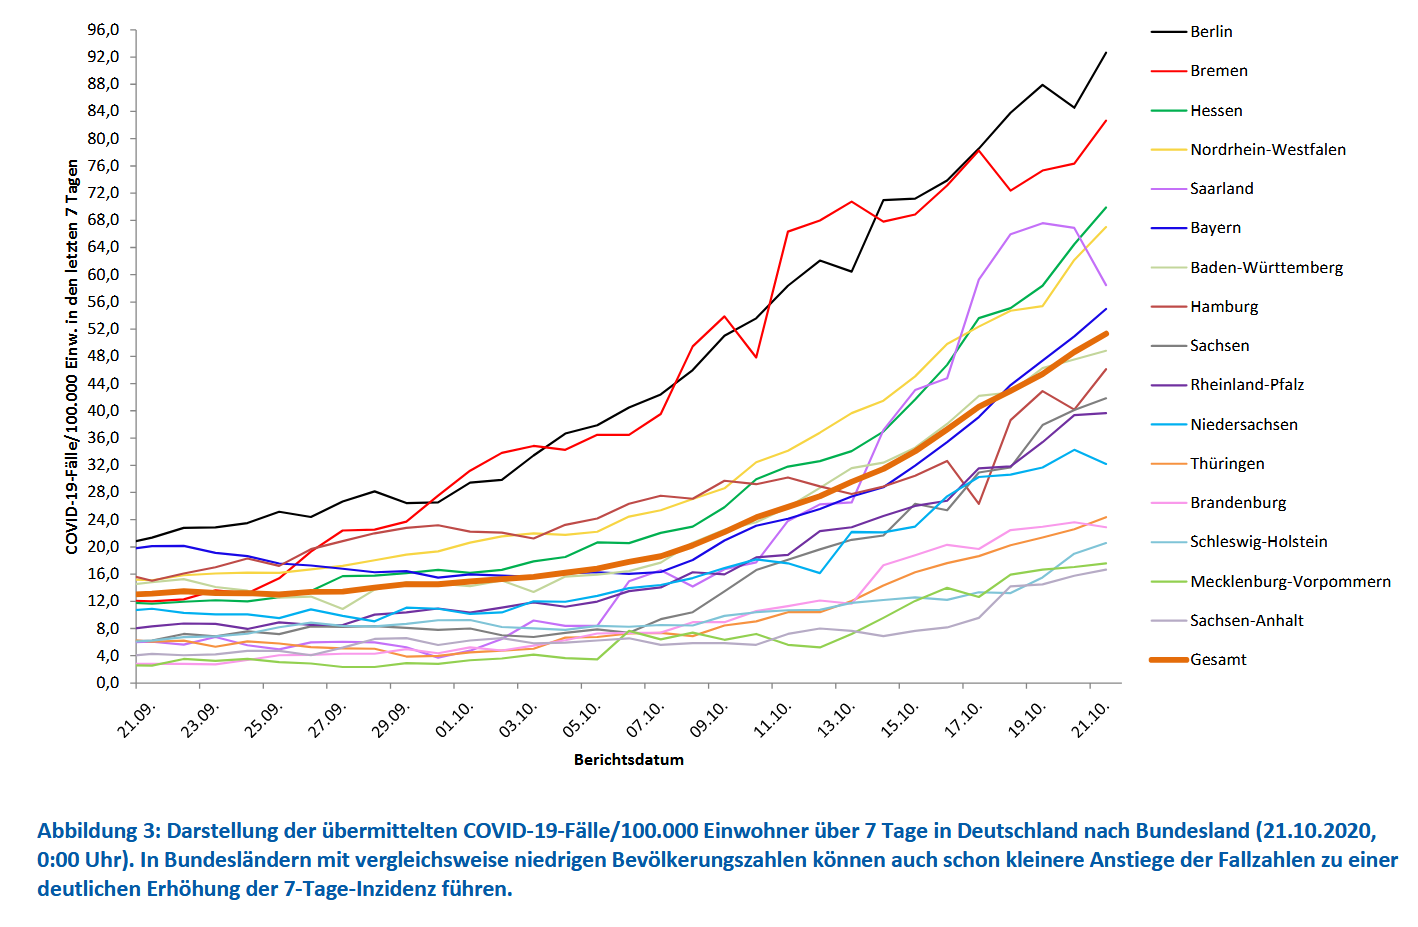
\includegraphics[keepaspectratio]{img/corona_okt_2020_germany.png}}

}

\caption{Picture taken from ``Täglicher Lagebericht des RKI zur
Coronavirus-Krankheit-2019 (COVID-19) 21.10.2020''}

\end{figure}%

Infectious diseases are a threat to humanity: some have the ability to
easily spread from one person to others persons and infecting all of
mankind, some can be transmitted before the infectious persons knows
that he is sick, some have no cure and a high fatality rate, some are
able to spread long distances via air, water or food.

To combat infectious diseases mankind has developed numerous techniques
throughout the ages. On very important tool that is a prerequisite to
most count measures is infectious disease surveillance. Knowing what
happens when and how is one of the cornerstonse of every response. And
infectious disease surveillance does exactly that.

\bookmarksetup{startatroot}

\chapter*{Presentations}\label{presentations}
\addcontentsline{toc}{chapter}{Presentations}

\markboth{Presentations}{Presentations}

Generel presentations about infectious disease surveillance

\hfill\break

\section*{Einführung}\label{einfuxfchrung}
\addcontentsline{toc}{section}{Einführung}

\markright{Einführung}

\begin{longtable}[]{@{}
  >{\raggedright\arraybackslash}p{(\linewidth - 2\tabcolsep) * \real{0.5000}}
  >{\raggedright\arraybackslash}p{(\linewidth - 2\tabcolsep) * \real{0.5000}}@{}}
\toprule\noalign{}
\begin{minipage}[b]{\linewidth}\raggedright
Target
\end{minipage} & \begin{minipage}[b]{\linewidth}\raggedright
Description
\end{minipage} \\
\midrule\noalign{}
\endhead
\bottomrule\noalign{}
\endlastfoot
\href{1_Presentations/presentation_einfuehrung.html}{Presentation} & The
link to the presentation \\
Content & This presentation gives an introduction to surveillance
system. How it is defined, how it falls in the domain of general
surveillance, what its objectives are \\
Time & 90 Minutes \\
Language & German \\
Intended audience & Ärztinnen und Ärzte in Weiterbildung zum Facharzt
für öffentliches Gesundheitswesen. \\
Learning objectives & (1) Surveillance ist wichtiger denn je (2) ``Daten
für Taten'' (3) Schritte der Surveillance (4) Surveillance muss
durchdefiniert werden \\
\end{longtable}

\section*{Introduction to surveillance
systems}\label{introduction-to-surveillance-systems}
\addcontentsline{toc}{section}{Introduction to surveillance systems}

\markright{Introduction to surveillance systems}

\begin{longtable}[]{@{}
  >{\raggedright\arraybackslash}p{(\linewidth - 2\tabcolsep) * \real{0.5000}}
  >{\raggedright\arraybackslash}p{(\linewidth - 2\tabcolsep) * \real{0.5000}}@{}}
\toprule\noalign{}
\begin{minipage}[b]{\linewidth}\raggedright
Target
\end{minipage} & \begin{minipage}[b]{\linewidth}\raggedright
Description
\end{minipage} \\
\midrule\noalign{}
\endhead
\bottomrule\noalign{}
\endlastfoot
\href{1_Presentations/presentation_introduction.html}{Presentation} &
The link to the presentation \\
Content & This presentation gives an introduction to surveillance
system. How it is defined, how it falls in the domain of general
surveillance, what its objectives are \\
Time & 15 Minutes \\
Language & English \\
Intended audience & Young professionals, Fellows of the European
programme for intervention epidemiology \\
Learning objectives & (1) Know the important parts of the definition (2)
Understand the domain surveillance (3) Know the objectives \\
\end{longtable}

\section*{Stages of surveillance
systems}\label{stages-of-surveillance-systems}
\addcontentsline{toc}{section}{Stages of surveillance systems}

\markright{Stages of surveillance systems}

\begin{longtable}[]{@{}
  >{\raggedright\arraybackslash}p{(\linewidth - 2\tabcolsep) * \real{0.5000}}
  >{\raggedright\arraybackslash}p{(\linewidth - 2\tabcolsep) * \real{0.5000}}@{}}
\toprule\noalign{}
\begin{minipage}[b]{\linewidth}\raggedright
Target
\end{minipage} & \begin{minipage}[b]{\linewidth}\raggedright
Description
\end{minipage} \\
\midrule\noalign{}
\endhead
\bottomrule\noalign{}
\endlastfoot
\href{1_Presentations/presentation_stages.html}{Presentation} & The link
to the presentation \\
Content & This presentation gives an overview of the stages of an
surveillance system. \\
Time & 10 Minutes \\
Language & English \\
Intended audience & Young professionals, Fellows of the European
programme for intervention epidemiology \\
Learning objectives & (1) Understand that the definition of surveillance
includes most stages (2) The stages are: Events, Collection,
Classification, Data management, Analysis, Communication, Action \\
\end{longtable}

\section*{Types of surveillance
systems}\label{types-of-surveillance-systems}
\addcontentsline{toc}{section}{Types of surveillance systems}

\markright{Types of surveillance systems}

\begin{longtable}[]{@{}
  >{\raggedright\arraybackslash}p{(\linewidth - 2\tabcolsep) * \real{0.5000}}
  >{\raggedright\arraybackslash}p{(\linewidth - 2\tabcolsep) * \real{0.5000}}@{}}
\toprule\noalign{}
\begin{minipage}[b]{\linewidth}\raggedright
Target
\end{minipage} & \begin{minipage}[b]{\linewidth}\raggedright
Description
\end{minipage} \\
\midrule\noalign{}
\endhead
\bottomrule\noalign{}
\endlastfoot
\href{1_Presentations/presentation_types.html}{Presentation} & The link
to the presentation \\
Content & This presentation gives an overview of the types of
surveillance system e.g.~case based, syndromic, event based, wastewater,
active vs passive \\
Time & 20 Minutes \\
Language & English \\
Intended audience & Young professionals, Fellows of the European
programme for intervention epidemiology \\
Learning objectives & (1) Understand that different overlapping types of
surveillance system exist (2) Know what case based surveillance is (3)
Know what syndromic surveillance is (4) Know what event based
surveillance is \\
\end{longtable}

\section*{Attributes of surveillance
systems}\label{attributes-of-surveillance-systems}
\addcontentsline{toc}{section}{Attributes of surveillance systems}

\markright{Attributes of surveillance systems}

\begin{longtable}[]{@{}
  >{\raggedright\arraybackslash}p{(\linewidth - 2\tabcolsep) * \real{0.5000}}
  >{\raggedright\arraybackslash}p{(\linewidth - 2\tabcolsep) * \real{0.5000}}@{}}
\toprule\noalign{}
\begin{minipage}[b]{\linewidth}\raggedright
Target
\end{minipage} & \begin{minipage}[b]{\linewidth}\raggedright
Description
\end{minipage} \\
\midrule\noalign{}
\endhead
\bottomrule\noalign{}
\endlastfoot
\href{1_Presentations/presentation_attributes.html}{Presentation} & The
link to the presentation \\
Content & This presentation covers the attributes of a surveillance
system. It covers underestimation, validty, timeliness and other
attributes \\
Time & 20 Minutes \\
Language & English \\
Intended audience & Young professionals, Fellows of the European
programme for intervention epidemiology \\
Learning objectives & (1) Be able to describe characteristics of a
surveillance system (2) Understand underestimation (3) Understand
validity (4) Understand timeliness (5) Know that there are many
attributes often with unclear defintions \\
\end{longtable}

\section*{Evaluation of surveillance
systems}\label{evaluation-of-surveillance-systems}
\addcontentsline{toc}{section}{Evaluation of surveillance systems}

\markright{Evaluation of surveillance systems}

\begin{longtable}[]{@{}
  >{\raggedright\arraybackslash}p{(\linewidth - 2\tabcolsep) * \real{0.5000}}
  >{\raggedright\arraybackslash}p{(\linewidth - 2\tabcolsep) * \real{0.5000}}@{}}
\toprule\noalign{}
\begin{minipage}[b]{\linewidth}\raggedright
Target
\end{minipage} & \begin{minipage}[b]{\linewidth}\raggedright
Description
\end{minipage} \\
\midrule\noalign{}
\endhead
\bottomrule\noalign{}
\endlastfoot
\href{1_Presentations/presentation_evaluation.html}{Presentation} & The
link to the presentation \\
Content & This presentation gives an overview of how to evaluate a
surveillance system. \\
Time & 10 Minutes \\
Language & English \\
Intended audience & Young professionals, Fellows of the European
programme for intervention epidemiology \\
Learning objectives & (1) Learn the steps of an evaluation (2) need to
adapt the evaluation to the trigger and the attributes (3) Surveillance
is a team effort \\
\end{longtable}

\part{Introduction}

\chapter{Definition of surveillance}\label{definition-of-surveillance}

Surveillance is information for action!

\hfill\break

The motto of public health surveillance ist information for action. This
is also the shortest definition of surveillance but does not capture all
elements. A history of the definitions can be found in the Article
\href{https://www.ncbi.nlm.nih.gov/pmc/articles/PMC3820481/table/tab5/}{The
Past, Present, and Future of Public Health Surveillance} by Bernard
Choi. The most influential definition is from Alexander Langumir that
set out the path for the future definitions.

\section{Definition of Public health surveillance by
WHO}\label{definition-of-public-health-surveillance-by-who}

\begin{quote}
Public health surveillance is an \emph{ongoing}, \emph{systematic}
\emph{collection}, \emph{analysis} and \emph{interpretation} of
health-related data essential to the planning, \emph{implementation},
and evaluation of public health practice. \footnote{World Health
  Organisation 2005 -
  https://www.ncbi.nlm.nih.gov/pmc/articles/PMC3820481/table/tab5/}
\end{quote}

\section{Important parts of the
definition}\label{important-parts-of-the-definition}

The definition of public health surveillance is very informative. It
gives us all important elements of a surveillance system.

\begin{longtable}[]{@{}
  >{\raggedright\arraybackslash}p{(\linewidth - 2\tabcolsep) * \real{0.2500}}
  >{\raggedright\arraybackslash}p{(\linewidth - 2\tabcolsep) * \real{0.7500}}@{}}
\caption{Elements of the public health surveillance
definition}\tabularnewline
\toprule\noalign{}
\begin{minipage}[b]{\linewidth}\raggedright
Element
\end{minipage} & \begin{minipage}[b]{\linewidth}\raggedright
Explanation
\end{minipage} \\
\midrule\noalign{}
\endfirsthead
\toprule\noalign{}
\begin{minipage}[b]{\linewidth}\raggedright
Element
\end{minipage} & \begin{minipage}[b]{\linewidth}\raggedright
Explanation
\end{minipage} \\
\midrule\noalign{}
\endhead
\bottomrule\noalign{}
\endlastfoot
ongoing & surveillance is planned for a longer time (usually). This is
in contrast to a scientific study or a survey \\
systematic & surveillance is a planned undertaking that works with clear
definitions \\
collection & Events are collected and stored in datasystems \\
analysis & Indicators are calculated and the data is parsed according to
time, place and person \\
interpretation & Assessment of the indicators and sense making \\
implementation of public health practice & The information guides public
health responses \\
\end{longtable}

\section{Infectious disease
surveillance}\label{infectious-disease-surveillance}

The infectious disease surveillance is that part of public health
surveillance that is concerned with the surveillance of infectious
diseases.

\chapter{Other forms of surveillance}\label{other-forms-of-surveillance}

What is the larger picture of surveillance?

\hfill\break

Nearly all complex biological and technical systems have mechanisms to
monitor and control the system's condition. Many social systems also
regularly analyze their current state. There are various terms for these
status assessments: A scientific study is one form of status assessment,
as is the police surveillance of a group or the evaluation of a project
in the corporate sector. Surveillance is also a form of status
assessment.

\section{Neighbourhood surveillance}\label{neighbourhood-surveillance}

Neighbourhood surveillance is the oldest form of surveillance. In its
broadest sense it es people watching other people. Small Communities
such as villages usually have a strong neighbourhood surveillance.
Neighbors see and know everything what other neigbohrs are doing. This
can be framed positively as in the saying: ``it takes a village to raise
a child'' or negatively when people blaspheme other people.

With the widespread availability of cameras and the possibility to
communicate directly this form of surveillance has gained a large
momentum. The largely unsuccesfull Google glass project could have been
an even larger driver of participatory surveillance. Now Surveillance
becomes a tool that does not lie in the hands of a strong actor such as
a state or less strong actors such as companies but in the hands of the
individuals. This gives infectious disease specialists the opportunity
to gather information from thos eindividuals as it is done in epidemic
intelligence.

This form of surveillance is sometimes also called participatory
surveillance - if you want to emphasize the empowerment of the people.
One rather negative example of a participatory surveillance is vividly
depicted in the book and film the circle. Sometimes this form of
surveillance is called bottom-up-surveillance to emphasize the
opposition to top-down-surveillance.

\section{Rhizomatic surveillance}\label{rhizomatic-surveillance}

Rhizomatic surveillance is a term coined by Haggerty and
Ericson\footnote{Haggerty KD, Ericson RV. The surveillant assemblage. Br
  J Sociol. 2000 Dec;51(4):605-22. doi: 10.1080/00071310020015280.
  \url{https://pubmed.ncbi.nlm.nih.gov/11140886/}}. The term comes from
rhizom - the large underground network from Fungi. This form of
surveillance shows similar characteristics of the rhizom: is is being
not directly visible (being ``underground'')), it is horizontal in
contrast to the top-down surveillance (like the rhizom that does not
follow the typical direction of plants growing upwards to the sun)) and
the surveillance is a group of different actors instead of one single
responsible body. The surveillance done by the big tech companies is a
form a rhizomatic surveillance. Collecting millons of datapoints that
are left behind by users in the internet can give valuable inside that
can be turned into profit. The cambridge analytica scandal is an example
of such a surveillance system. State actors are of course also capable
of doing rhizomatic survaillance as could bee seen in the documents
leaked to PRISM.

\section{Top-down-surveillance}\label{top-down-surveillance}

The top-down-surveillance is the surveillance which we usually think of
first when we hear the word surveillance. There is an agent usually a
dominent one like the state who watches was its constituents do. This
can take the form of an Panopticon, where one person can watch many
different person and after which some prisons have been modeled. This
form of surveillance often aims to achieve a specific behavior among
those being monitored. Epidemiological surveillance belongs to this
level of surveillance.

\section{Learn more}\label{learn-more}

You can read more about different types of surveillance in this article
by Tieman et al.~\footnote{ Timan, Tjerk and Galič, Maša and Koops,
  Bert-Jaap, Surveillance Theory and Its Implications for Law (December
  1, 2017)
  \url{https://papers.ssrn.com/sol3/papers.cfm?abstract_id=3098182}}

\chapter{International regulations}\label{international-regulations}

How is surveillance regulated internationally

\hfill\break

\section{International health
regulations}\label{international-health-regulations}

Surveillance is firmly anchored in national and international legal
systems. The
\href{https://www.who.int/health-topics/international-health-regulations}{International
Health Regulations} (IHR) is a legally binding regulation for 196
countries. The IHR includes articles that require surveillance from the
countries. The aim is to prevent cross-border threats from infectious
diseases.

During the COVID-19 pandemic, the value of such international
collaboration became evident. New amendments of the IHR were adopted on
the first of June 2024. It will come into place in 2025/2026.

\begin{figure}[H]

{\centering \pandocbounded{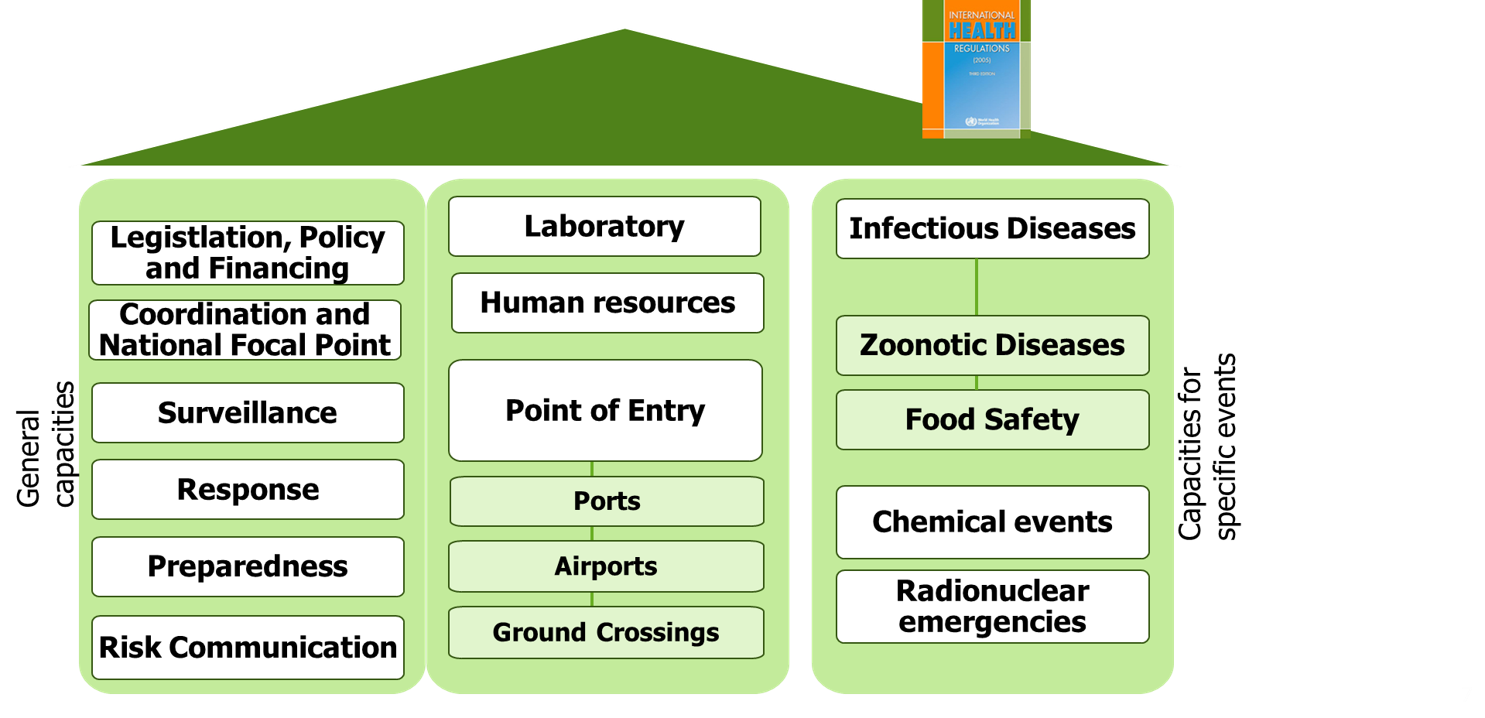
\includegraphics[keepaspectratio]{2_Introduction/../img/background_ihr.png}}

}

\caption{Contents of the IHR. Graph by ÖGD-Kontaktstelle RKI}

\end{figure}%

\subsection{Important contents of the
IHR}\label{important-contents-of-the-ihr}

\begin{itemize}
\tightlist
\item
  The IHR defines a Public Health Emergency of International Concern
  (PHEIC). It is defined as an extraordinary event which is determined
  to constitute a public health risk to other states and potentially
  requires a coordinated international response
\item
  A PHEIC is declared by the Director General of WHO
\item
  Notification accoring to Article 6 Annex 2: Sate Parties to notify WHO
  withing 24 hours about events within their terriory wich can consitute
  a PHEIC
\item
  Article 8: State Parties can seek consultation from WHO
\item
  Article 10: WHO can request State Parties to verify an event and offer
  to collaborate on this event. States are obliged to give information
  within 24h
\item
  \href{https://iris.who.int/bitstream/handle/10665/246107/9789241580496-eng.pdf?sequence=1}{Annex
  2}: Decision tool for deciding if an event should be notified. It
  consists of a flowchart with 4 questions. There are
  \href{https://www.who.int/publications/m/item/annex-2-of-the-international-health-regulations-(2005)}{helpful
  ressources to learn how to use the annex 2}
\item
  The IHR Monitoring and Evaluation Framework provides an overview of
  approaches to review implementation of country core public health
  capacities under the IHR (2005)
\item
  The
  \href{https://www.who.int/emergencies/operations/international-health-regulations-monitoring-evaluation-framework}{Monitoring
  and evaluation framework} describes mandatory and voluntary approaches

  \begin{itemize}
  \tightlist
  \item
    IHR State Party Self-Assessment annual report (mandatory)
  \item
    simulation exercises (voluntary)
  \item
    after action reviews (voluntary)
  \item
    joint external evaluation (voluntary)
  \end{itemize}
\end{itemize}

\subsection{History of PHEICS}\label{history-of-pheics}

\begin{itemize}
\tightlist
\item
  2009: H1N1 Pandemic
\item
  2014: Resourgence of Polio
\item
  2014: Ebola Westafrica
\item
  2016: Zika
\item
  2019: KIVU Ebola
\item
  2020: SARS-CoV-2
\item
  2022: Clade II Mpox
\item
  2024: Clade I Mpox
\end{itemize}

\section{EU Regulation 2022/2371}\label{eu-regulation-20222371}

\begin{itemize}
\tightlist
\item
  The EU has its own regulation on infectious diseases
\item
  Regulation on serious cross-border threats to health
\item
  Content:

  \begin{itemize}
  \tightlist
  \item
    Establishing a health security committee
  \item
    reference laboratory networks
  \item
    surveillance
  \item
    network for substances of human origin
  \end{itemize}
\item
  Mandatory events to notify in the Early warning and response system
  (EWRS)

  \begin{itemize}
  \tightlist
  \item
    unusual or unexpected, may cause significant morbidity or mortality
    in humans, may grow rapidly in scale,
  \item
    may exceed national response capacity;
  \item
    may affect more than one Member State; and
  \item
    may require a coordinated response at Union level
  \item
    Anything they notified to WHO via Annex 2
  \end{itemize}
\end{itemize}

\section{Essential public health
operations}\label{essential-public-health-operations}

Surveillance is also a component of the
\href{https://who-sandbox.squiz.cloud/en/health-topics/Health-systems/public-health-services/policy/the-10-essential-public-health-operations}{Essential
Public Health Operations}. The essential public health regulations are a
tool of WHO Europe and defines central tasks for public health
institutes. The goal of this
\href{https://who-sandbox.squiz.cloud/en/health-topics/Health-systems/public-health-services/policy/the-10-essential-public-health-operations/epho1-surveillance-of-population-health-and-wellbeing}{surveillance
component} is to provide information and insights for health needs
assessments, health impact assessments, and the planning of health
services.

\part{Stages}

\chapter{Objectives of surveillance (Stage
1)}\label{objectives-of-surveillance-stage-1}

If you are clear about your objectives everything will be easier.

\hfill\break

\pandocbounded{\includegraphics[keepaspectratio]{3_Stages/../img/surveillance_plots/surveillance_en_stage1.pdf}}

The objectives of a surveillance system are the reasons why a
surveillance systems is set into place. The overall objective of
infectious disease surveillance is described nicely in the German
infection protection act:

\begin{quote}
prevent communicable diseases in humans, detect infections at an early
stage, and prevent their further spread\footnote{Translated from the
  German infection protection act
  \url{https://www.gesetze-im-internet.de/ifsg/__1.html}}
\end{quote}

The overarching objectiv can be decomposed into more conrete objectives
that are based on the interventions that can be taken. These can be
subdivided into primary objectives that have a direct effect on the
spread of an infectious disease or secondary objectives that exert and
indirect influence.

\section{Primary objectives}\label{primary-objectives}

\begin{longtable}[]{@{}
  >{\raggedright\arraybackslash}p{(\linewidth - 2\tabcolsep) * \real{0.5000}}
  >{\raggedright\arraybackslash}p{(\linewidth - 2\tabcolsep) * \real{0.5000}}@{}}
\toprule\noalign{}
\begin{minipage}[b]{\linewidth}\raggedright
Objective
\end{minipage} & \begin{minipage}[b]{\linewidth}\raggedright
Description
\end{minipage} \\
\midrule\noalign{}
\endhead
\bottomrule\noalign{}
\endlastfoot
Get information to initate case based action & All the interventions
that are taken when there is a person with an infection \\
Get information to initate population based action & All the
interventions that are taken that affect a large part of the
population \\
Get information to initate individual action & interventions taken by
the individual \\
Get information to initate action by medical professionals & The
interventions that are taken by the medical system. A special form of
the individual action \\
\end{longtable}

\section{Secondary objectives}\label{secondary-objectives}

\begin{longtable}[]{@{}
  >{\raggedright\arraybackslash}p{(\linewidth - 2\tabcolsep) * \real{0.5000}}
  >{\raggedright\arraybackslash}p{(\linewidth - 2\tabcolsep) * \real{0.5000}}@{}}
\toprule\noalign{}
\begin{minipage}[b]{\linewidth}\raggedright
Objective
\end{minipage} & \begin{minipage}[b]{\linewidth}\raggedright
Description
\end{minipage} \\
\midrule\noalign{}
\endhead
\bottomrule\noalign{}
\endlastfoot
Scientific advances & Advance the knowledge on infectious diseases \\
Evaluation & Documents the impact of an intervention, or track progress
towards specified goals \\
Resource allocation & Set priorities by the governmant or an institution
and develope long term strategy \\
Fullfill obligation & Most nations have commited themselves to the
International Health regulations. Thus they have to set up surveillance
system \\
\end{longtable}

\section{Get information to initate case based
action}\label{get-information-to-initate-case-based-action}

Many public health interventions focus around the direct prevention of
the spread from one person to another. This action is usually taken by a
local public health agency. For this a surveillance systems needs to
directly identify the single cases. So the objective of the surveillance
system is to get all necessary information.

\section{Get information to initate population based
action}\label{get-information-to-initate-population-based-action}

Some public health interventions focus on the population or a group.
These interventions are sometimes described as
non-pharmaceutical-interventions - although this sometimes also
compromises case based interventions. This kind of intervention is often
done via a regulation by a federal state or a national body. But it can
also be taken by a local public health agency. This action requires
usually only trends and not necessariliy case based information. So a
surveillance system can have the objective to get the necessary
information for this action

\section{Get information to initate individual
action}\label{get-information-to-initate-individual-action}

The information from surveillance systems can lead to people changing
their behaviour. This compromises many different interventions, that are
taken by the people themselves (if it is initatied by an agency it would
be a population based intervention). These interventions can be
ineffective or even counterproductive. So the surveillance can have the
objective to elicit the information that is needed from the individuals
to do effective and useful action.

\section{Get information to initate action by medical
professionals}\label{get-information-to-initate-action-by-medical-professionals}

Some findings of surveillance systems lead to a change in practice of
medical professionals. A medical professional society could change the
guidelines according to findings. This intervention is initiated by the
medical people and not necessarily by the public health agencies. The
objective of the surveillance could be based on eliciting the
information needed.

\section{Scientific advances}\label{scientific-advances}

Surveillance systems collect data that can also be used for public
health research. Scientists can use the data to analyse specific public
health problems. The system can give information about the nature of a
pathogen and epidemiological characteristics of a public health problem.
One example would be the change of variants that follow the introduction
of a new vaccine.

\section{Evaluation}\label{evaluation}

Public health interventions should be benefical for the population. The
intervention can measure output, outcome and impact. Measuring the
impact can be considered the most important part because it shows the
benefits. This impact measurement can be done in with a surveillance
system.

\section{Resource allocation}\label{resource-allocation}

Governments need to decide about their priorities and the distribution
of resources. These decisions can be taken upon the information from
surveillance systems.

\section{Fullfill obligation}\label{fullfill-obligation}

The International health regulations require: \emph{Each State Party
shall develop, strengthen and maintain {[}\ldots{]} the capacity to
detect, assess, notify and report events} Thus it can be an objective of
a surveillance system to fullfill these obligations.

\section{Other concepts for
objectives}\label{other-concepts-for-objectives}

There are other summaries for the objectives of a surveillance system
that have a similar concepts.

\subsection{World bank}\label{world-bank}

The world bank notes the objectives of an public health surveillance
system as follows\footnote{https://documents1.worldbank.org/curated/en/239131468160515361/pdf/536490BRI0ENGL10Box345621B01PUBLIC1.pdf}:\\
\emph{- recognize cases or clusters of cases to trigger interventions to
prevent transmission or reduce morbidity and mortality (includes the
special case in which surveillance at the national level is required to
recognize multi-state clusters); - identify new health problems and
emerging diseases; - assess public health impact of health events or
determine and measure trends; - measure causal factors in disease (e.g.,
risk factors) to initiate actions to prevent the onset of disease; -
demonstrate the need for intervention programs and resources, and
allocate resources during health planning; - monitor effectiveness and
evaluate the impact of prevention and control measures, intervention
strategies, and health policy changes; - identify high-risk population
groups or geographic areas to target interventions and guide analytic
studies; - provide data for research, and develop hypotheses that lead
to analytic studies about risk factors for disease causation,
propagation or progression; - measure progress toward Millennium
Development Goals, or other project or program goals, including PRSP
(Poverty Reduction Strategy Paper) targets.}

\subsection{EU/EEA surveillance}\label{eueea-surveillance}

The EU/EEA surveillance \footnote{https://www.ecdc.europa.eu/sites/default/files/documents/long-term-surveillance-framework-2021-2027.pdf}
focuses on the need for the supranational body - Detect and monitor any
multinational infectious disease outbreaks with respect to source, time,
population, and place in order to provide a rationale for public health
action; - Monitor trends in infectious diseases over time and across
Member States to assess the present situation, respond to rises above
warning thresholds and facilitate appropriate evidence-based action; -
Contribute to the evaluation and monitoring of prevention and control
programmes targeted at infectious diseases in order to provide the
evidence for recommendations to strengthen and improve these programmes
at the national and European level; - Identify population groups at risk
and in need of targeted prevention measures; - Contribute to the
awareness of and the assessment of the burden of infectious diseases on
the population using such data as disease prevalence, complications,
hospitalisation, and mortality; and - Generate hypotheses on (new)
sources, modes of transmission and groups most at risk and identify
needs for research and pilot projects

\section{Objectives in practice}\label{objectives-in-practice}

Although objectives play a decisive role in theory they are not as
relevant in practice. Large surveillance systems tend to develope a life
on its own and the focus on the objectives gets lost over time. New
changes are introduced based on new needs but old parts stay in place
although they might have losts their importance.

\chapter{Infection Event (Stage 2)}\label{infection-event-stage-2}

Choosing the right event is crucial and depends on the objectives

\hfill\break

\pandocbounded{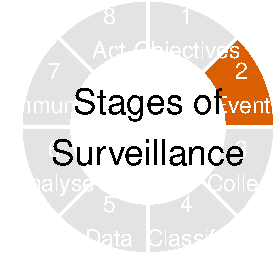
\includegraphics[keepaspectratio]{3_Stages/stage2_files/figure-pdf/unnamed-chunk-1-1.pdf}}

Surveillance systems monitor a wide range of infection-related events.
Understanding the event is essential for understanding a surveillance
system.The choice of events to monitor in a surveillance system is a
critical decision that shapes the system's in many ways. The choice
depends on the Objective of the surveillance system.

\begin{itemize}
\tightlist
\item
  If a case-based intervention is intended the event that is monitored
  should be able to provide contact information of a case
\item
  If only goup-based intervention is inteded only a trend is needed
  which can be acquired by simpler systems
\item
  When the objective of a surveillance system is to monitor hospital
  capacity for resource allocation decisions, the events tracked should
  focus on specific indicators of hospital capacity and utilization like
  bed occupancy of staff coverage.
\end{itemize}

\section{Naming and Categorization}\label{naming-and-categorization}

Surveillance systems are often named after the events they monitor. For
example:

\begin{itemize}
\tightlist
\item
  Emergency department surveillance (Emergency department visits)
\item
  Syndromic surveillance (based on monitoring syndromes)
\item
  Lab-based surveillance system (Reports by labs)
\item
  Meidasurveillance (Screening of media articles)
\end{itemize}

\section{Typical events in infectious disease
surveillance}\label{typical-events-in-infectious-disease-surveillance}

\begin{itemize}
\tightlist
\item
  The occurence of an infectious disease
\item
  The occurence of an infection (infected person who is not necessarily
  diseased)
\item
  An available ICU bed
\item
  Self reports by people that they fell sick
\item
  The colonization of a person by a pathogen
\item
  A physician's ICD-10 classification of a patient
\item
  The discovery of a newspaper article about a disease outbreak
\item
  The subjective assessment of a public health department employee that
  something poses a threat to the population.
\item
  A social media signal detected by a software
\end{itemize}

\chapter{Collection (Stage 3)}\label{collection-stage-3}

With the collection method you will introduce the most important bias

\hfill\break

\pandocbounded{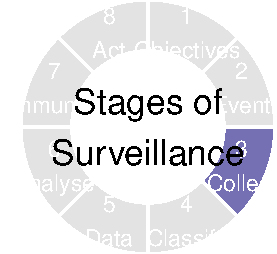
\includegraphics[keepaspectratio]{3_Stages/stage3_files/figure-pdf/unnamed-chunk-1-1.pdf}}

The collection of an infectious disease Event form the foundation of any
effective surveillance. The specific methods of collection can vary
widely depending on the type of surveillance system. The collection is
usually done by an public health agency or a commisioned insitution. The
method of data collection often influences the naming of surveillance
systems.

A collection processes can be based on any comminication form like:
Phone calls, serial interface, Reports on paper, Fax or E-Mail, direct
investigation. In recent years many efforts have been put into
establishing a fully seamless electronic system via electronic
interfaces.

\section{Typical collection methods}\label{typical-collection-methods}

\begin{itemize}
\tightlist
\item
  Physicians report diagnosed cases to health authorities.
\item
  Laboratories report cases that are analysed for clinical purposes to
  public health agencies
\item
  Laboratories report cases that are analyses specifically for public
  health puropses like sequencing data to public health agencies
\item
  Laboratories report other lab results like PCR-tests in wastewater
\item
  A pulic health agency follows-up on an initial reports.
\item
  Health insurance claims and ICD-10 Codes are collected via a software
  interface
\item
  A public health agency gets access to a database of death records
\item
  Public health workers go around households in a crisis situation and
\item
  Hospital representatives fill out an online form about the number of
  free intensive care beds
\item
  A specific group uses a software that screens the internet for
  potential public health threats
\item
  Blood prodocuts are analysed for infectious disease
\end{itemize}

\section{Active vs.~passive}\label{active-vs.-passive}

The collection process can be described as active or passive. Where
active means that the public health agency actively collect reports,
whereas passive means, that public health agency recieve reports and
dont directly interfere in the reporting. Many collection methods
contain both, e.g.~reports are sent in by a lab (passive) but in
relevant cases the agency reaches out to get more information about a
specific case (active)

\begin{longtable}[]{@{}lll@{}}
\toprule\noalign{}
Characteristic & Active & Passive \\
\midrule\noalign{}
\endhead
\bottomrule\noalign{}
\endlastfoot
Ease & Complicated & Easy \\
Speed & slow & fast \\
Scalability & low & high \\
Operational costs & high & low \\
External validity & high & low \\
\end{longtable}

\section{Enhanced and intensived}\label{enhanced-and-intensived}

If there are several events that are looked at, that are collected via
different methods the term: ``enhanced'' or ``intensivied'' are used,
especially in a mass-gathering surveillance.

\section{Integreated and one-health}\label{integreated-and-one-health}

If collection methods by veteniary or food-safety agencies are included
the term ``integrated'' or ``one-health'' is applied.

\chapter{Classification (Stage 4)}\label{classification-stage-4}

Clear definitions are crucial and avoids creating rubbish

\hfill\break

\pandocbounded{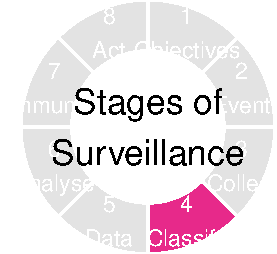
\includegraphics[keepaspectratio]{3_Stages/stage4_files/figure-pdf/unnamed-chunk-1-1.pdf}}

\begin{tcolorbox}[enhanced jigsaw, opacitybacktitle=0.6, titlerule=0mm, breakable, bottomrule=.15mm, colframe=quarto-callout-warning-color-frame, toprule=.15mm, left=2mm, colbacktitle=quarto-callout-warning-color!10!white, coltitle=black, colback=white, bottomtitle=1mm, rightrule=.15mm, toptitle=1mm, title=\textcolor{quarto-callout-warning-color}{\faExclamationTriangle}\hspace{0.5em}{Warning}, opacityback=0, arc=.35mm, leftrule=.75mm]

The content of this chapter is the personal opionon of the author. This
is escpecially true for the discouragment of the usage of the word case
definition\_\_

\end{tcolorbox}

Classification means categorizing the recorded events into two or more
groups. Sometimes the word ``collation'' is used for this stage, for
example in the WHO definition of surveillance. Classification means a
person or software applies a set of uniform criteria to define a
disease, health event or condition for infectious disease surveillance.
The classification is based on the specific objective.\\
Usually the word ``applying a case definition'' is used to describe this
process. But it is better to use more specific words and use the word
``case definition'' for the general concept. Classification is often a
hidden part of the surveillance system or built into the system in a way
that it is not recognized as such. For example, the application of
reporting definition is built into the reporting software.\\
Definitions enable public health officials to classify and count cases
consistently for example across reporting jurisdictions. This avoids
comparing ``apples to oranges''. Classification is important because
recorded events can be erroneous and should not be counted. Or there may
not be enough information to decide whether a real event has occurred.
Without classification, the events form an unclear collection with
questionable significance. Even in seemingly trivial classifications,
important definitions must be agreed upon: In a mortality surveillance
deaths are counted. But does the death of a tourist with a foreign
passport count as a death in the surveillance system?

\section{Typical classification
definitions}\label{typical-classification-definitions}

\begin{longtable}[]{@{}
  >{\raggedright\arraybackslash}p{(\linewidth - 2\tabcolsep) * \real{0.2500}}
  >{\raggedright\arraybackslash}p{(\linewidth - 2\tabcolsep) * \real{0.7500}}@{}}
\caption{Typical definitions used in surveillance
systems}\tabularnewline
\toprule\noalign{}
\begin{minipage}[b]{\linewidth}\raggedright
Definition
\end{minipage} & \begin{minipage}[b]{\linewidth}\raggedright
Description
\end{minipage} \\
\midrule\noalign{}
\endfirsthead
\toprule\noalign{}
\begin{minipage}[b]{\linewidth}\raggedright
Definition
\end{minipage} & \begin{minipage}[b]{\linewidth}\raggedright
Description
\end{minipage} \\
\midrule\noalign{}
\endhead
\bottomrule\noalign{}
\endlastfoot
\textbf{Reference definition} & A reference definition is used for
official reporting (e.g.~national yearly reporting) \\
\textbf{Case-finding definition} & A case-finding definition is applied
for an the search of cases in an outbreak \\
\textbf{Notification definition} & A notification definition is applied
by physisicans or labs whether they should notify a diseases person \\
\textbf{Reporting definition} & A reporting definition is applied by
local public health agencies before reporting a case to a state or
national level \\
\textbf{Intervention definition} & A intervention definition is applied
when to act upon an information \\
\textbf{ECDC case definition} & The ECDC case definitions are used for
the reports of ECDC \\
\textbf{Outbreak-study definition} & An outbreak study definition is
used for a cohort or case-study \\
\textbf{Suspected case definition} & This definition is used in an
outbreak response \\
\textbf{Probable case definition} & This definition is used in an
outbreak response \\
\textbf{Confimed case definition} & This definition is used in an
outbreak response \\
\textbf{Contact definition} & This definition is used in an outbreak
response \\
\textbf{Clinical definition} & A clinical definition is applied when
someone in the medical systems uses his or her knowledge whether this
constitutes a disease \\
\textbf{ICD-10 definition} & A medical classification system that is
especiall used for the reimbursment of physicians \\
\textbf{Infected person} & Somebody who inoculated a pathogen, that
subsequently replicates within the body \\
\textbf{Diseased person} & Somebody with an infection with any kind of
symptoms that are caused by the infection process. \\
\end{longtable}

Example for the application of definitions along the surveillance stages
of a case-based surveillance system.

\subsection{Example of the different usages of
definitions}\label{example-of-the-different-usages-of-definitions}

A person inoculates hepatitis B virus and the pathogen subsequently
replicates in the body of the person (Fullfilling the infection
definition). He then develops symptoms (therby fullfilling the diseased
person definition) and he seeks the help of a doctor who gives him
treatment (apllying a clinical definition) and enters the data into his
software for reimbursment (applying the ICD-10 defintion). The physician
notifies the local public health agency because the law requires to
notify all diseased patients with acute hepatitis B (the notification
definition). The local public health agency then decides to act
(implicitly applying an intervention definition). They ensue an outbreak
investigation and look for cases and contacts (applying case finding
definitions or contact definitions). The local public health agency
enters the data into their notification software that applies an
algorithm and identifies that this event should be reported to the state
and national agencies (reporting definition). The national agency
reports the case in their official report (applying the referen
definition). The software scripts in the national agency find that the
event should be reported to ECDC (applying the ECDC case definition)

\section{Components of definitions}\label{components-of-definitions}

Typical definitions in the field of infectious diseases include some or
all of the following components

\begin{longtable}[]{@{}
  >{\raggedright\arraybackslash}p{(\linewidth - 2\tabcolsep) * \real{0.2500}}
  >{\raggedright\arraybackslash}p{(\linewidth - 2\tabcolsep) * \real{0.7500}}@{}}
\caption{Components of definitions}\tabularnewline
\toprule\noalign{}
\begin{minipage}[b]{\linewidth}\raggedright
Component
\end{minipage} & \begin{minipage}[b]{\linewidth}\raggedright
Explanation
\end{minipage} \\
\midrule\noalign{}
\endfirsthead
\toprule\noalign{}
\begin{minipage}[b]{\linewidth}\raggedright
Component
\end{minipage} & \begin{minipage}[b]{\linewidth}\raggedright
Explanation
\end{minipage} \\
\midrule\noalign{}
\endhead
\bottomrule\noalign{}
\endlastfoot
Time & The timeframe in which a disease is looked at (in surveillance
systems this is often missing) \\
Place & Where a disease is looked at. E.g. a region \\
Person & Who is looked at. It can be everybody in a certain region or it
can be only a specific group in an outbreak session \\
Clinical & Include common and relevant signs and symptoms of the disease
under surveillance Form either individually or in combination a clear or
indicative picture of the disease \\
laboratory & Includes a list with methods used to confirm the pathogen
Usually: One of the laboratory methods on the list is sufficient for
confirmation of a disease \\
Epidemiological criteria & Are met when an epidemiological link is
established Depending on: Incubation period of the disease Transmission
Routes (person-to-person, contaminated food, \ldots) Endemicity of the
disease in the country \\
\end{longtable}

\subsection{Example for a clinical part of a case
defintion}\label{example-for-a-clinical-part-of-a-case-defintion}

\begin{figure}[H]

{\centering \pandocbounded{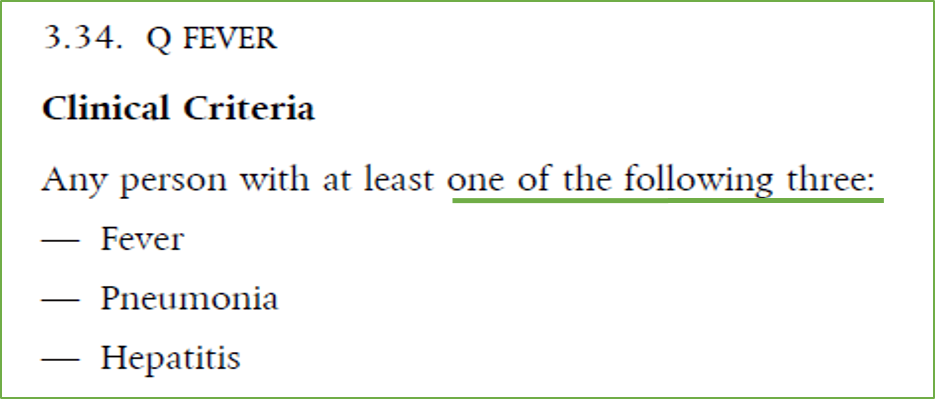
\includegraphics[keepaspectratio]{3_Stages/../img/stages_casedefinitions_qfever.png}}

}

\caption{Case definition for Q-Fever by the european center for disease
control}

\end{figure}%

\subsection{Example for a laboratory part of a case
defintion}\label{example-for-a-laboratory-part-of-a-case-defintion}

\begin{figure}[H]

{\centering \pandocbounded{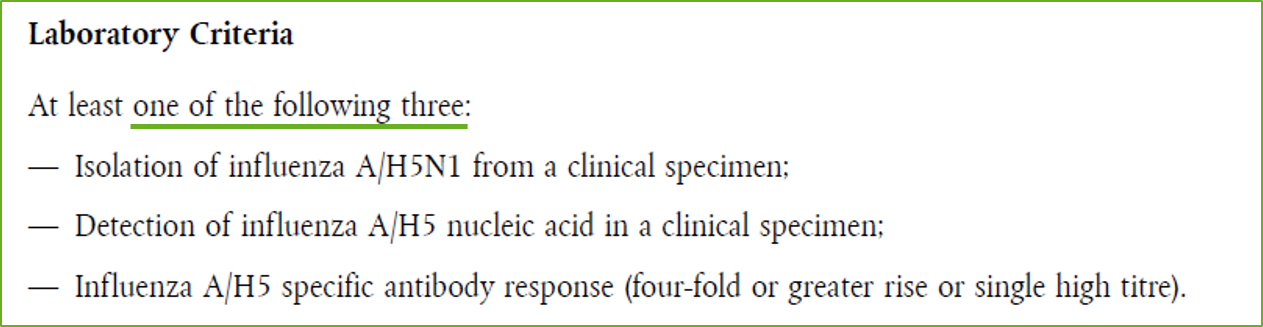
\includegraphics[keepaspectratio]{3_Stages/../img/stages_casedefinitions_avian.png}}

}

\caption{Case definition for avian flu by the european center for
disease control}

\end{figure}%

\subsection{Example for an epidemiological part of a case
defintion}\label{example-for-an-epidemiological-part-of-a-case-defintion}

\begin{figure}[H]

{\centering \pandocbounded{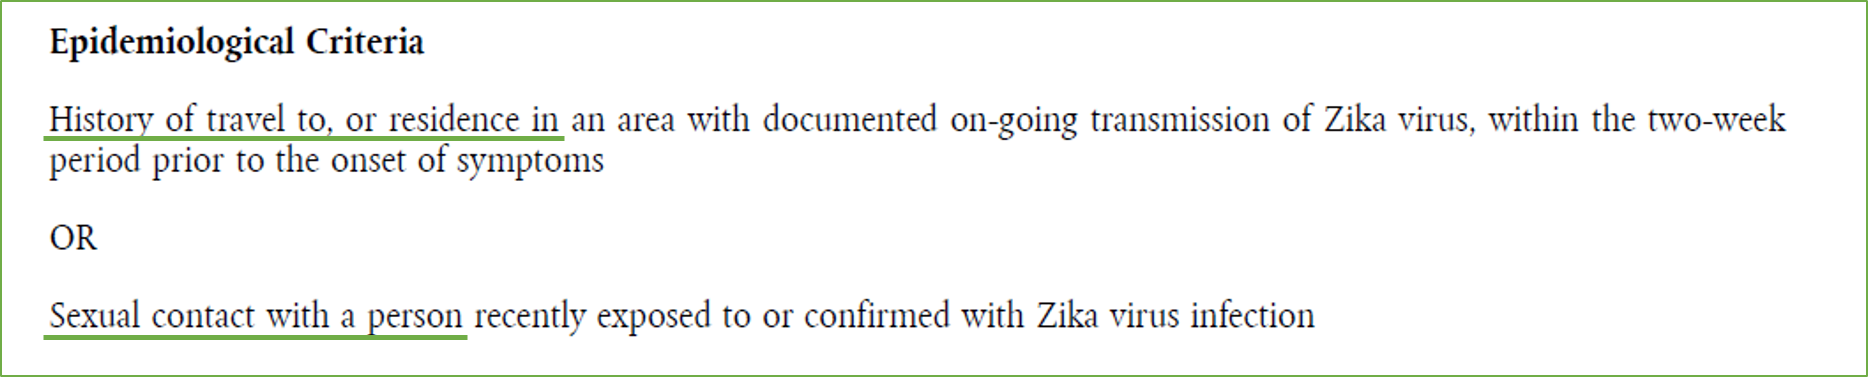
\includegraphics[keepaspectratio]{3_Stages/../img/stages_casedefinitions_zika.png}}

}

\caption{Case definition for zika by the european center for disease
control}

\end{figure}%

\section{Specificity and sensitvity}\label{specificity-and-sensitvity}

\begin{itemize}
\tightlist
\item
  A definition can be sensitive or specific. Sensitive means that more
  events are captured but likely this will increase the number of
  wrongly identified events. Specific means that less events are
  captured but the number of wrongly identified events is lower.
\end{itemize}

\section{Creating you own
definitions}\label{creating-you-own-definitions}

\begin{itemize}
\tightlist
\item
  Identify the objectives of the surveillance system
\item
  Involve a multi-sectoral team (e.g.~physicians, reference
  laboratories, epidemiologists,\ldots)
\item
  Balance between sensitivity and specificity when collecting /
  reporting
\item
  Define important and frequently used terms (e.g.~fever)
\item
  Use a standardised format and structure for all case definitions
\item
  Plan the implementation of the case definitions (e.g.~communicate,
  train, evaluate)
\end{itemize}

\chapter{Data Processing (Stage 5)}\label{data-processing-stage-5}

The data processing is where you spend your time in infectious disease
surveillance

\hfill\break

\pandocbounded{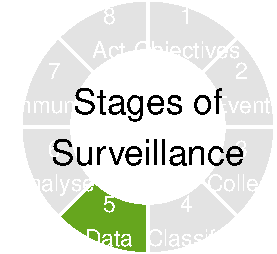
\includegraphics[keepaspectratio]{3_Stages/stage5_files/figure-pdf/unnamed-chunk-1-1.pdf}}

Data processing is seldom mentioned in classical surveillance
literature, but it is a stage that significantly improves surveillance
systems. Many people at all levels are involved in data processing
within surveillance systems. In the past, data was transmitted monthly
by mail in surveillance systems, whereas today, data flow mostly occurs
through interfaces between software programs and databases. The way data
is transmitted affects data quality and, consequently, the evaluation of
the data. Data processing also includes the application of scripts that
prepare the data for subsequent evaluation. An example is automated
outbreak detection. Here, data is analyzed using an algorithm or machine
learning to determine whether there is a high probability of an
outbreak. The resulting dataset can be made available as open data, a
publication format that has increased significantly in recent times.

\section{Typical ways of data
processing}\label{typical-ways-of-data-processing}

\begin{itemize}
\tightlist
\item
  Questionnaires on paper
\item
  Software interface between laboratory information system and public
  health notification software
\item
  Accessing a database via an API
\item
  Querying persons with a survey app
\item
  Keeping information in a large excel sheet
\end{itemize}

\section{Comparing characteristics of manual vs electronic data
processing}\label{comparing-characteristics-of-manual-vs-electronic-data-processing}

\begin{longtable}[]{@{}lll@{}}
\toprule\noalign{}
Characteristic & Manual & Electronic \\
\midrule\noalign{}
\endhead
\bottomrule\noalign{}
\endlastfoot
Ease & Easy & Complicated \\
Internal validity & Low & High \\
Speed & slow & fast \\
Scalability & low & high \\
Setup costs & low & high \\
Operational costs & high & low \\
Accepatbility & low & high \\
Understandability & high & low \\
\end{longtable}

\section{Problems of data processing}\label{problems-of-data-processing}

\subsection{Dependence on the user interface of
software}\label{dependence-on-the-user-interface-of-software}

The interface of the software that is used influences the data. If the
variables that need to be entered are placed on different spots and
described differently than one can expect different results

\subsection{Dependence on classification systems in manual
systems}\label{dependence-on-classification-systems-in-manual-systems}

\subsection{Dependence on classification systems in automatic
systems}\label{dependence-on-classification-systems-in-automatic-systems}

\begin{itemize}
\tightlist
\item
  SnowMed
\item
  FIHR
\end{itemize}

\subsection{Single point of truth}\label{single-point-of-truth}

\subsection{Errors in data handling by the
software}\label{errors-in-data-handling-by-the-software}

\begin{itemize}
\tightlist
\item
  Excel changes specific values to dates automatically
\item
  Excel sheets have only a certain number of rows
\end{itemize}

\section{Open Data and Public
Engagement}\label{open-data-and-public-engagement}

Recent trends in data publication have expanded assessment beyond
designated experts:

Advantages:

Enables independent verification Increases transparency Potentially
leads to novel insights

Challenges:

Risk of misinterpretation by non-experts Necessitates clear
communication of data limitations and context

Control group must be - representative of exposures in the source
population - be identifiable as cases - habe same exclusion and
restctition criteria as cases

\chapter{Analysis and Assessment (Stage
6)}\label{analysis-and-assessment-stage-6}

Be true to yourself

\hfill\break

\pandocbounded{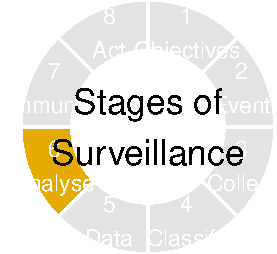
\includegraphics[keepaspectratio]{3_Stages/stage6_files/figure-pdf/unnamed-chunk-1-1.pdf}}

The analysis and assessment stage involves the calculation of relevant
indicators, examining data through the lenses of time, place, and
person, assessing the results by drawing of conclusions and eventually
formulating recommendations. Essentially, this stage transforms raw data
into actionable information, aligning with the
``data--information--knowledge--wisdom'' hierarchy\footnote{Rowley, J.
  (2007). The wisdom hierarchy: representations of the DIKW hierarchy.
  Journal of Information Science, 33(2), 163-180.
  \url{https://doi.org/10.1177/0165551506070706}}.

The complexity of analysis varies significantly across scenarios:

\begin{itemize}
\tightlist
\item
  Straightforward cases: Some situations demand immediate action based
  on clear indicators. For instance, a reported case of Ebola in a
  returning traveler unequivocally signals the need for prompt
  intervention.
\item
  Complex scenarios: Other situations require nuanced interpretation and
  extensive expertise. For example, determining whether a relative
  increase in a SARS-CoV-2 variant warrants action involves intricate
  analysis and often necessitates collaborative evaluation among
  experts.
\end{itemize}

\section{Analysis}\label{analysis}

\subsection{Surveillance indicators}\label{surveillance-indicators}

The analysis process begins with data from the processing stage,
typically structured in spreadsheets or databases. From this foundation,
surveillance indicators are computed based on the specific objectives of
the surveillance system. Here are key indicators often used in health
surveillance:

\begin{longtable}[]{@{}
  >{\raggedright\arraybackslash}p{(\linewidth - 2\tabcolsep) * \real{0.2500}}
  >{\raggedright\arraybackslash}p{(\linewidth - 2\tabcolsep) * \real{0.7500}}@{}}
\caption{Typical indicators used in surveillance systems}\tabularnewline
\toprule\noalign{}
\begin{minipage}[b]{\linewidth}\raggedright
Indicator
\end{minipage} & \begin{minipage}[b]{\linewidth}\raggedright
Description
\end{minipage} \\
\midrule\noalign{}
\endfirsthead
\toprule\noalign{}
\begin{minipage}[b]{\linewidth}\raggedright
Indicator
\end{minipage} & \begin{minipage}[b]{\linewidth}\raggedright
Description
\end{minipage} \\
\midrule\noalign{}
\endhead
\bottomrule\noalign{}
\endlastfoot
Count & Total number of cases meeting the relevant definition \\
Incidence proportion & Probability that a particular event has occurred
in a specified period. \\
Incidence rate & Frequency of new occurrences of a medical disorders in
the studied population at risk of the medical disorder arising in a
given period of time. \\
Prevalence proportion & Proportion of a defined population affected by a
particular medical disorder at a given point in time, or over a
specified period of time \\
Hospiatlisation rate & Incidence rate for cases of a disease that are
hospitalised \\
\end{longtable}

\subsection{Graphical Display}\label{graphical-display}

In addition to computing indicators, data visualization plays a crucial
role in making complex information easily interpretable. Graphs
transform raw data into visual representations that are readily
understood by humans. Common examples in infectious disease surveillance
include:

\begin{itemize}
\tightlist
\item
  Epidemic curves (Epicurves): Showing the progression of cases over
  time
\item
  Dot maps: Illustrating the geographic distribution of cases
\end{itemize}

\subsection{Time, Place, Person}\label{time-place-person}

Infectious disease data is typically analyzed across three key
dimensions:

\begin{itemize}
\tightlist
\item
  Time:

  \begin{itemize}
  \tightlist
  \item
    Data is arranged chronologically to reveal temporal patterns.
  \item
    Example: Epicurves showing the number of cases per day or week.
  \end{itemize}
\item
  Place:

  \begin{itemize}
  \tightlist
  \item
    Data is categorized by geographic distribution.
  \item
    In outbreak settings: Dot maps or incidence maps are created.
  \item
    In routine surveillance: Indicators are computed separately for each
    subregion.
  \end{itemize}
\item
  Person:

  \begin{itemize}
  \tightlist
  \item
    Demographic factors: Age, sex
  \item
    Social factors: Occupation
  \item
    Epidemiological characteristics: Risk factors, vaccination status
  \end{itemize}
\end{itemize}

\subsection{Process}\label{process}

While manual analysis can be preferred in outbreak settings for rapid
information gathering, the computation of indicators and production of
graphs is typically automated using software. Common tools include:

\begin{itemize}
\tightlist
\item
  Spreadsheet applications (e.g., Excel)
\item
  Statistical software packages (e.g., R, Stata)
\end{itemize}

\section{Assessment}\label{assessment}

After the data has been analyzed across time, place, and person
dimensions, experts evaluate the resulting indicators and graphs. This
assessment process is inherently subjective and context-dependent,
involving several key aspects:

\begin{itemize}
\tightlist
\item
  Interpretation of Patterns:

  \begin{itemize}
  \tightlist
  \item
    Analyzing graph shapes and indicator values
  \item
    Identifying and investigating outliers (data points that deviate
    from typical patterns)
  \end{itemize}
\item
  Contextual Analysis:

  \begin{itemize}
  \tightlist
  \item
    Incorporating relevant literature and evidence
  \item
    Considering information from other surveillance systems and sources
  \item
    Understanding system limitations (e.g., changes in testing
    strategies affecting case numbers)
  \end{itemize}
\item
  Holistic Evaluation:

  \begin{itemize}
  \tightlist
  \item
    Experts synthesize quantitative data with qualitative insights
  \end{itemize}
\end{itemize}

\subsection{Formulating of public health
recommendations}\label{formulating-of-public-health-recommendations}

Sometimes the information found in a surveillance system can lead to
public health recommendations

\subsection{Recommendations (post-evidence)}

\begin{tcolorbox}[enhanced jigsaw, opacitybacktitle=0.6, titlerule=0mm, breakable, bottomrule=.15mm, colframe=quarto-callout-warning-color-frame, toprule=.15mm, left=2mm, colbacktitle=quarto-callout-warning-color!10!white, coltitle=black, colback=white, bottomtitle=1mm, rightrule=.15mm, toptitle=1mm, title=\textcolor{quarto-callout-warning-color}{\faExclamationTriangle}\hspace{0.5em}{Warning}, opacityback=0, arc=.35mm, leftrule=.75mm]

Warning: This is the personal opinion of the author and not the standard
theory

\end{tcolorbox}

\begin{itemize}
\tightlist
\item
  Base recommendations on evidence, where evidence is available and do
  not give recommendations that contradict evidence
\item
  Demphasize areas where evidence is available and emphasise areas where
  evidence is not available
\item
  Convey uncertainty
\item
  Formulate recommendations with diverse experts
\item
  Try to create more options in the future
\item
  Time your recommendations
\item
  Use gut-feeling, where gut-feeling is likely to be good
\item
  Fit recommendations to the world-view of people
\item
  Minimize harm
\end{itemize}

\subsection{Recommendations (evidence version)}

\begin{itemize}
\tightlist
\item
  Evidence-based (Evidence that the actions recommended will control the
  outbreak or improve health outcomes)
\item
  Specific (Prioritised clear list of actions that all targeted
  understand: Describe `what', `who', `when', `how')
\item
  Feasible (Logistics, willingness, systems, access, sustainable)
\item
  Acceptable
\item
  Cost-effective
\item
  Ethical
\end{itemize}

\chapter{Communication (Stage 7)}\label{communication-stage-7}

Communication in a complex world is difficult

\hfill\break

\pandocbounded{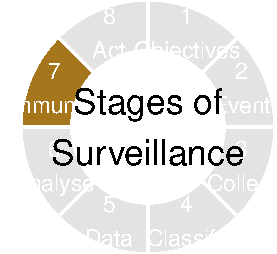
\includegraphics[keepaspectratio]{3_Stages/stage7_files/figure-pdf/unnamed-chunk-1-1.pdf}}

Communication is the dissemination of the obtained information in words,
writing, and images. Communication consists of traditional elements such
as press releases and press conferences or the preparation of reports.
Communication now also includes social media and fact-checking. The
presentation of data and information in dashboards also counts as
communication.

\section{Graphical}\label{graphical}

the graphical representation of information is often done in terms of
time, place, and person

The communication of epidemiological information was a major focus
towards the end of the pandemic and is an area with strong development
potential. Almost worldwide, a significant portion of the population
rejected the measures to combat the COVID-19 pandemic, thereby
influencing the course of the pandemic.

\chapter{Public Health Measures (Stage
8)}\label{public-health-measures-stage-8}

This is what its all about.

\hfill\break

\pandocbounded{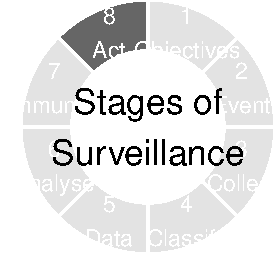
\includegraphics[keepaspectratio]{3_Stages/stage8_files/figure-pdf/unnamed-chunk-1-1.pdf}}

Measures are the goal towards which surveillance is directed. Public
health measures are all deliberate efforts by commissioned actors aimed
at preventing the further spread and generally minimizing the harm
caused by infectious diseases. Measures are often legally defined.
Measures can be divided into case-based measures and population-based
measures. Case-based measures include, for example, informing an
affected person about transmission routes or measures such as
quarantine. Population-based measures are those that affect many people,
for example, the population of a federal state.

Typical interventions taken are:\\
- guidance: The local public gives the case or his contact persons
guidance on what to do and how to behave - mandate: The local public
health official could order a case or a contact person to do something.
This could be quarantine for example - information: the local public
health agency informs everybody who needs to know about this public
health event

Typical population based interventions are: - Boiling water before
drinking - Requiring to wear masks - Closing schools - Giving advice

Typical interventions are: - change in calculated antibitotic therapy
(so before information about resistance of the specific pathogen is
available) according to a higher resistancy in an area - change in
immunization strategies

Typical interventions are: - Wearing masks - Washing handy frequently -
Not using public transport - Avoiding specific groups

\part{Types}

\chapter{Case based surveillance}\label{case-based-surveillance}

\begin{figure}

\begin{minipage}{0.20\linewidth}
\pandocbounded{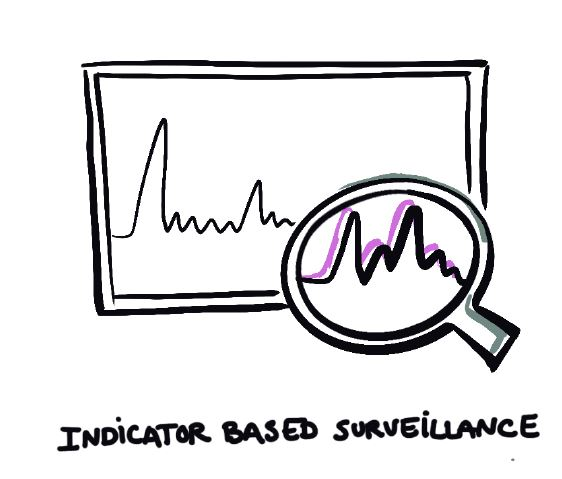
\includegraphics[keepaspectratio]{4_Types/../img/icons/indicator_based_surveillance.jpg}}\end{minipage}%
%
\begin{minipage}{0.80\linewidth}
A case-based surveillance system focuses on identifying persons that
have been diagnosed with an infectious diseases. A person diagnosed with
a disease is called a case if the appropriate definition is fullfilled
\href{../stages/stage4.qmd}{See the classification stage}. Case-based
surveillance is the most important type of infectious diesase
surveillance.\end{minipage}%

\end{figure}%

\section{Terminology}\label{terminology}

A case-based surveillance system is also called an indicator-based
surveillance\footnote{The surveillance of communicable diseases in the
  European Union -- a long-term strategy (2008-2013)
  https://www.eurosurveillance.org/images/dynamic/EE/V13N26/art18912.pdf}
It is called indicator to convey that the focus lies on the compilation
of indicators. The term case-based surveillance is - in the eyes of the
author of this book - more accurate as it puts the focus on the event
under surveillance which distinguishes it from other types of
surveillance systems. Other surveillance systems also compile indicators
e.g.~the viral load in wastewatersurveillance. The CDC usually describes
the concept as a case surveillance but less frequently also as a
notification-based surveillance system\footnote{https://www.cdc.gov/nndss/about/index.html}.
This type is sometimes refferd to as physician-based surveillance or
lab-based surveillance when physicians or labs are the main provider of
information.

\section{Process of a case-based surveillance
system}\label{process-of-a-case-based-surveillance-system}

As case-based surveillance is normally mandated by law, the objectives
are often laid down during the legislative process. A typical process is
that a physician is required to fill out a form when she or he finds a
person that has a disease. The form is then send to a local public
health agency where the event is collected and classified. The local
public health agency takes appropriate measures and enters the data into
a software. This data is transferred to regional or national levels
where experts analyse the data for the reporting and supraregional
measures.

\begin{figure}[H]

{\centering \pandocbounded{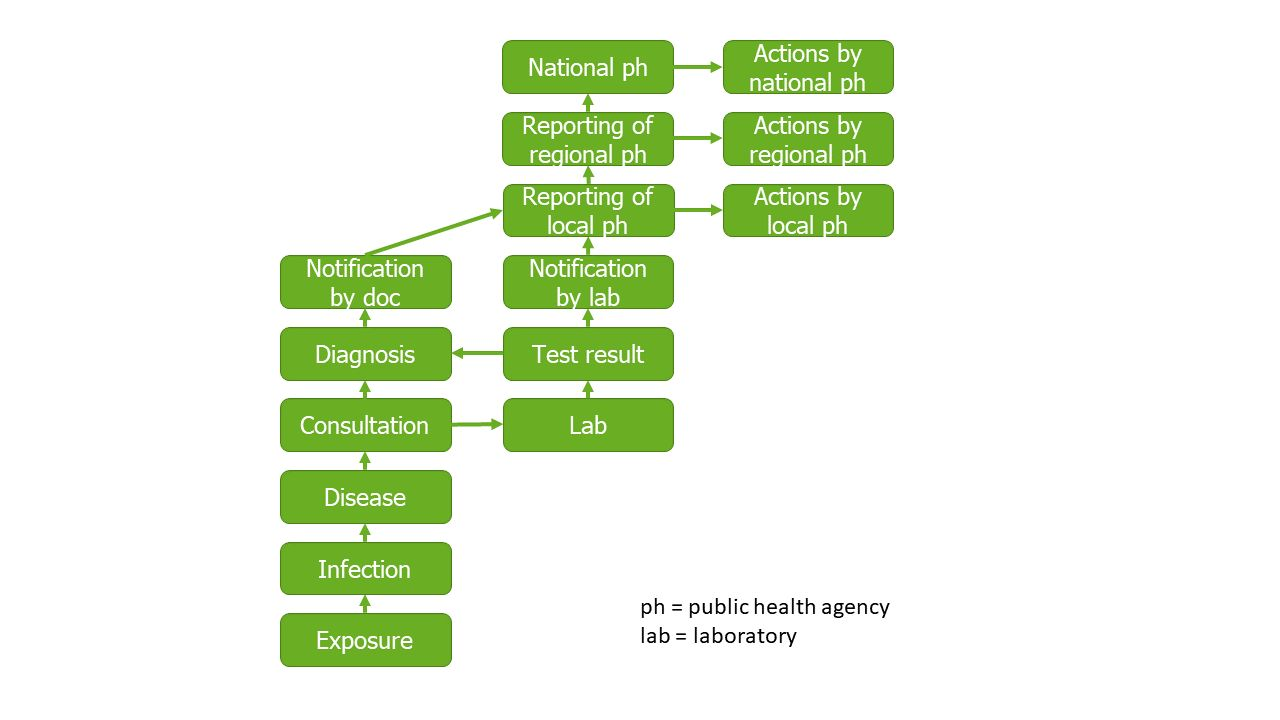
\includegraphics[keepaspectratio]{4_Types/../img/types_scope.jpg}}

}

\caption{Scope of a case based surveillance system. Adapted from ECDC
Handbook Data quality monitoring and surveillance system evaluation}

\end{figure}%

\section{Strengths and weaknesses}\label{strengths-and-weaknesses}

Strengths:\\
- measures one central event in infectious diseases directly - allows
case-based measures - allows collecting detailed information e.g.~on
exposure or demographics - usually allows the measurment of the severity
of a disease (e.g.~hospitalisation)

Weaknesses:\\
- usually goes along with a strong selection bias, especially in disease
with a many asymptomatic cases - expensive - depends on a reliable
health system

\section{Example of a case based surveillance
system}\label{example-of-a-case-based-surveillance-system}

The German infectious disease reporting system is governed by the
Infection Protection Act (IfSG). It is the backbone of epidemiological
surveillance in Germany. It has developed historically and has its roots
in the Imperial Epidemic Act of 1900. This act hat for example the
following regulation: \emph{``Any case of illness and any death from
leprosy, cholera (Asian), typhus, yellow fever, plague (Oriental bubonic
plague), smallpox {[}\ldots{]} must be reported immediately to the
competent police authority.''} The current reporting system was
established in 2000 with the creation of the Infection Protection Act.
The reporting system is legally regulated in Sections 6 to 11 of the
Act, which have been amended multiple times, usually in response to
acute events such as the HUS epidemic in 2011.

The events (Stage 1) monitored are typically the occurrence of
infectious diseases. However, the reporting system encompasses various
reporting obligations and multiple reporting channels. It can therefore
be viewed as a collection of related but essentially different
surveillance systems. A significant component of the reporting system is
the obligation for physicians, pathologists, and other professionals to
report. The event captured in this context is the suspicion of a
disease, the diagnosis of the disease, or the death from a diseases. The
infectious diseases are laid out in the text of the law and consists out
of severe diseases that can be medically diagnosed, such as measles,
polio, or HUS. Another relevant component is the obligation for
laboratories to report. The monitored event is a laboratory finding
indicative of an acute infection. This laboratory reporting obligation
applies to a wide range of infectious diseases. In addition to the
physician and laboratory reporting obligations, there are other
components, such as non-nominal reporting obligations for the laboratory
detection of certain pathogens like HIV, which follow a separate
reporting pathway.

The capture of physician and laboratory reports (Stage 2) is usually
carried out through the reporting process and investigations by the
health authorities. For many years, the method of reporting was not
standardized and was typically done via fax. In the last decade, the
German Electronic Reporting and Information System (DEMIS) has been
developed, primarily digitizing the reporting process from the reporter
to the health authority. This method of reporting is now legally
required for many reporting channels under the Infection Protection Act.
The way health authorities conduct investigations is not prescribed,
although there are, of course, restrictions due to privacy rights. A
common investigation involves a phone call from the health authority and
an infection control interview with the affected individuals. The
reporting system is thus a hybrid system of passive and active
surveillance. It is passive because the monitored events do not exist
solely because of the reporting system. For instance, in most cases, a
laboratory test is performed for clinical reasons, not for
epidemiological reasons. It is active because health authorities
actively investigate and contact the affected individuals. Investigation
is a central part of the job profile for public health inspectors.

The classification (Stage 3) within the reporting system is performed by
the health authority, assisted by the respective reporting software.
After entering the collected data, the software indicates whether the
event matches the defined criteria. These definitions are twofold:
first, there is a definition for events that must be reported to the
state authority and the RKI (``reporting definition''), and second,
there is a definition for cases officially counted in the RKI statistics
(``reference definition''). Establishing these definitions is crucial
for ensuring comparability and identifying increases or decreases in the
number of cases. At the start of the COVID-19 pandemic, the Chinese
government changed the case definition of COVID-19, leading to an
artificial spike in the statistics. Case definitions can be sensitive,
aiming to capture as many cases as possible, or specific, aiming to
include only a small number of false-positive cases. Case definitions
exist not only for a surveillance system but are also often established
separately for outbreaks. Additionally, case definitions are not
necessarily the standard for implementing measures. For example, in a
suspected case of hemorrhagic fever, action does not need to wait until
a case definition is met.

Data management (Stage 4) takes place after classification. The
reporting system has significantly benefited from more professional data
management. Before the introduction of electronic reporting software,
data was transmitted laboriously and prone to errors via mail or fax.
With increasing digitization and the reduction of media disruptions,
data management has become increasingly precise and faster. The most
well-known reporting software, SurvNet, from the Robert Koch Institute
(RKI), sets the standards for transmission from the health authority to
the state authority and from there to the RKI. Data management is
carried out in databases operated by the RKI. This process includes
quality assurance and data preparation for the subsequent evaluation
stage. The preparation also involves automated signal detection,
identifying and appropriately displaying potential outbreaks.

The analysis of the reporting system's data occurs at all three levels:
local, state, and national. This is similar to the interventions taken.
Usually the local agency takes case based measurements, whereas the
state and the nation take population-based measurements

\chapter{Syndromic Surveillance}\label{syndromic-surveillance}

Syndromic surveillance refers to surveillance systems where the relevant
event is not a diagnosed disease but rather cases from a group of
illnesses. So threats can be detected if if there is no specific
diagnosis yet. Syndromic surveillance can use many different events that
indicate a syndrom.

Typical events:

\begin{itemize}
\tightlist
\item
  Physician office visits
\item
  ICD-10 Codes of Hospitals
\item
  Self assessment of people
\item
  Information seeking
\item
  Prescriptions
\item
  Absenteeism
\end{itemize}

Advantages:

\begin{itemize}
\tightlist
\item
  can detect unkown or lesser-known diseases
\item
  syndromic systems can be very fast
\item
  can often be acquired automatically because it often works well with
  classification systems like ICD-10 codes
\end{itemize}

Disadvantages

\begin{itemize}
\tightlist
\item
  Syndromic surveillance is usually a sentinel system and not
  comprehensive
\item
  Difficult to interpret during high activities of several similar
  diseases
\item
  Calculating incidence and prevalence is usually biased because the
  denominator is not clear
\end{itemize}

Examples: For example, in syndromic surveillance, instead of tracking
cases of SARS-CoV-2 infection, cases of acute respiratory illness are
recorded. This approach makes the surveillance system more sensitive,
capturing a broader spectrum of diseases. When a signal suggests a
relevant event, such as an outbreak, further investigation can be
conducted to identify the exact pathogen.

\chapter{Event based surveillance}\label{event-based-surveillance}

How do we find public health threats that we did not anticipate?

\hfill\break

\textbf{Warning: This is not ready}

Event based surveillance is a defined system that rapidly detects events
that might be a threat to public health. These events could be news
reports, rumors, social media or informations by other surveillance
systems. The collected events are then analysed, assessed and the
relevent information is disseminated. The goal of an event based
surveillance system is to provide an early warning system and detect
previously unkown or generally threats, that are not detected by
indicator based surveillance systems.

\section{Stages of event based
surveillance}\label{stages-of-event-based-surveillance}

\section{Terminology}\label{terminology-1}

\subsection{Event based vs.~indicator based
surveillance}\label{event-based-vs.-indicator-based-surveillance}

The termin indicator based surveillance is opposite to event based
surveillance. Indicator based means that there are predifined indicators
that are monitored, for example a syndromic or case-based surveillance
system. When you look closely the line becomes somwhat blurred because
event based surveillance can also incooperate indicator based
surveillance.

\begin{longtable}[]{@{}
  >{\raggedright\arraybackslash}p{(\linewidth - 4\tabcolsep) * \real{0.1600}}
  >{\raggedright\arraybackslash}p{(\linewidth - 4\tabcolsep) * \real{0.4200}}
  >{\raggedright\arraybackslash}p{(\linewidth - 4\tabcolsep) * \real{0.4200}}@{}}
\caption{Characteristics of indicator and event based
surveillance}\tabularnewline
\toprule\noalign{}
\begin{minipage}[b]{\linewidth}\raggedright
Characteristic
\end{minipage} & \begin{minipage}[b]{\linewidth}\raggedright
Indicator based surveillance
\end{minipage} & \begin{minipage}[b]{\linewidth}\raggedright
Event based surveillance
\end{minipage} \\
\midrule\noalign{}
\endfirsthead
\toprule\noalign{}
\begin{minipage}[b]{\linewidth}\raggedright
Characteristic
\end{minipage} & \begin{minipage}[b]{\linewidth}\raggedright
Indicator based surveillance
\end{minipage} & \begin{minipage}[b]{\linewidth}\raggedright
Event based surveillance
\end{minipage} \\
\midrule\noalign{}
\endhead
\bottomrule\noalign{}
\endlastfoot
Process & Routine, Systematic, Pre-defined pathways and indicators &
Formalized, Ad hoc and in real time, Flexible \\
Data & Organized data with predefined variables, Trusted and reliable,
often health-care sector based & Not organized or predefined (variable),
Reliability to be assessed \\
Sources & Formal sources (usually one sector) & All sources
(Meida/Internet, Communication, Indicator based surveillance) \\
\end{longtable}

\subsection{Epidemic intelligence}\label{epidemic-intelligence}

Event based surveillance and epidemic intelligence are often used as
synonyms. But some argue that epidemic intelligence is broader than
event based surveillance to emphasize the fact that it also uses
indicator based surveillance and encompasses the verification,
assessment and investigation steps\footnote{https://www.eurosurveillance.org/content/10.2807/esm.11.12.00665-en}.
But as the usage of indicator based surveillance and steps of
verification, assessment and investigation also falls within the
definition of event based surveillance or surveillance in general, there
is no need to use the term epidemic intelligence.

\section{Strengths and weaknesses}\label{strengths-and-weaknesses-1}

Strengths:\\
- Can detect unkown or not-thought of public health threats - Is usually
fast - Has a formalised way of assessing risks

Weakness: - Large subjective component - Does not give reliable
statistical measurements (e.g.~trends)

\begin{tcolorbox}[enhanced jigsaw, leftrule=.75mm, colback=white, breakable, arc=.35mm, rightrule=.15mm, bottomrule=.15mm, colframe=quarto-callout-color-frame, opacityback=0, toprule=.15mm, left=2mm]

\textbf{Definition:} Event-based surveillance is the organized and rapid
capture of information about events that are a potential risk to public
health\footnotemark{}

\end{tcolorbox}

\footnotetext{https://iris.who.int/bitstream/handle/10665/207737/9789290613213\_eng.pdf?sequence=1}

\section{Sources of event based
surveillance}\label{sources-of-event-based-surveillance}

\begin{figure}[H]

{\centering \pandocbounded{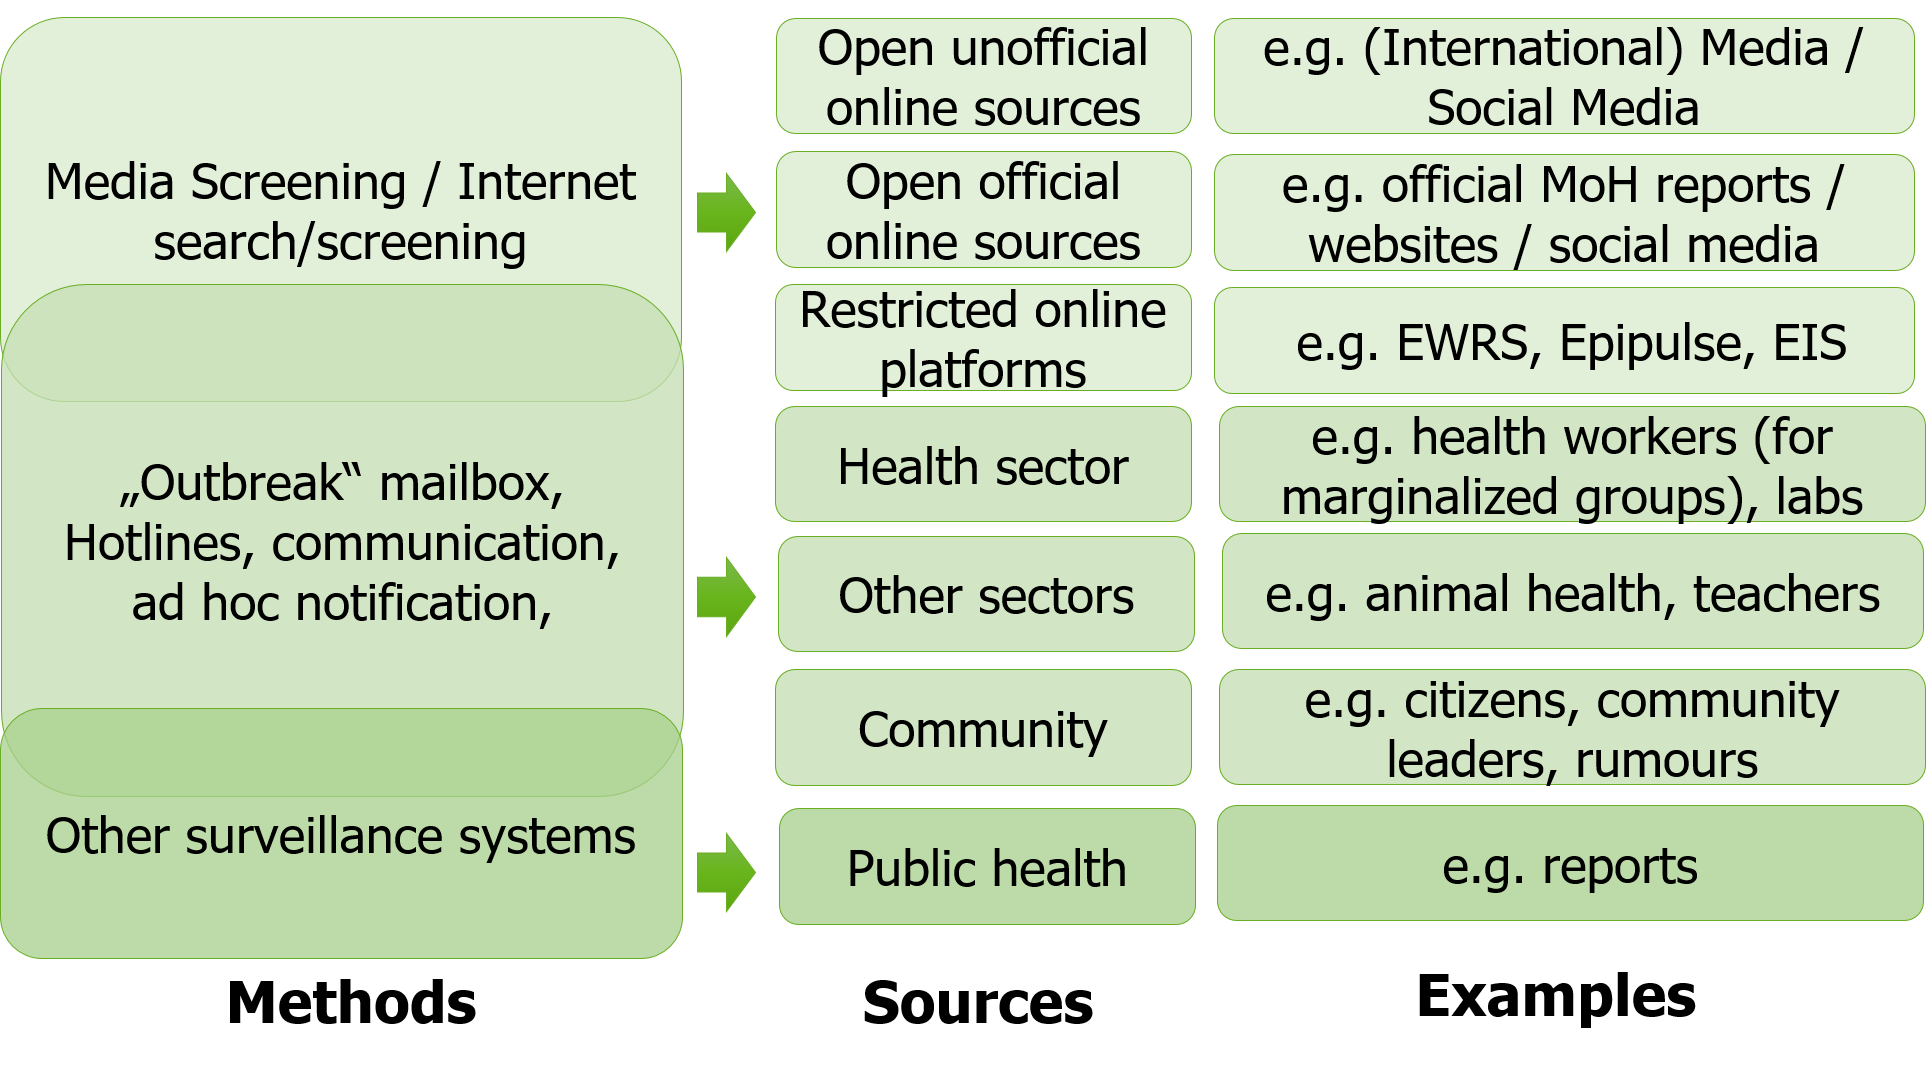
\includegraphics[keepaspectratio]{4_Types/../img/types_event_sources.png}}

}

\caption{Graph adapted from the ECDC Fellowship programme}

\end{figure}%

\section{}\label{section}

An example of such surveillance is an expert commission that regularly
meets to collect potentially relevant events.

\section{Resources}\label{resources}

\begin{itemize}
\tightlist
\item
  \href{https://www.ncbi.nlm.nih.gov/pmc/articles/PMC10712973/}{Norzin
  T, Ghiasbeglou H, Patricio M, Romanova S, Zaghlool A, Tanguay F, Zhao
  L. Event-based surveillance: Providing early warning for communicable
  disease threats. Can Commun Dis Rep.~2023 Feb 1;49(1):29-34. PMID:
  38090144}
\end{itemize}

\chapter{Wastewater}\label{wastewater}

Wastewatersurveillance is a system that measures indicators of diseases
in wastewater. Pathogens can be excreted via stool, urine or washed into
the drain during shower. These pathogens can be detected at a
wastewatertrement plant.

\chapter{Mortality surveillance}\label{mortality-surveillance}

Mortality surveillance asses the number of deaths. One example would be
the collection of deaths certificates by physicians. They are legally
required to fill out a form after a person dies. These forms are
collected by specific agencies and the number of deaths or the reasons
for death can be analysed by public health experts.

\chapter{Mass-Gathering Surveillance}\label{mass-gathering-surveillance}

Mass-gathering surveillance refers to surveillance systems that are set
up for the duration of a special event. A mass-gathering is a planned or
spontaneous event where the number of people attending could strain the
planning and response resources of the community or country hosting the
event\footnote{WHO Definition of mass-gathering.
  https://www.who.int/news-room/questions-and-answers/item/what-is-who-s-role-in-mass-gatherings}

Mass-gatherings can be a threat to public health because any large group
of people poses the risk of the spread of an infectious disease. Such
events are also accomapnied by many small food vendors, that have
limited facilites. As many mass-gathering usually go along with lots of
international attention and the attention of media, there is usually a
political pressure.

Typically, different components from other surveillance systems are
employed. For instance, a separate surveillance system might be
implemented during a European Football Championship.

\section{Additional reading}\label{additional-reading}

\begin{itemize}
\tightlist
\item
  Mass gathering events and communicable diseases - Considerations for
  public health authorities
  \url{https://www.ecdc.europa.eu/sites/default/files/documents/Mass-gathering-events-and-communicable-diseases-June-2024.pdf}
\end{itemize}

\chapter{Active vs passive}\label{active-vs-passive}

Case based surveiallance systems can be divided whether they are active
or passive. Many surveillancesystems have elements of both.

\section{Active surveillance system}\label{active-surveillance-system}

An active surveillance system involves a group of individuals who
actively collect information for the surveillance system.

An example of an active surveillance system would if the staff of an
agency goes door-to-door to gather information.

\section{Passive surveillance system}\label{passive-surveillance-system}

A passive surveillance system uses data collected for other purpose.
Passive surveillance can be seen as secondary data analysis.

An example for a passive surveillance system could be a system that
extracts data from a hospital database.

\chapter{Sentinal vs comprehensive}\label{sentinal-vs-comprehensive}

Sentinel surveillance is a system that does not monitor all individuals
about whom conclusions are to be drawn but rather only a defined
portion. The term ``Sentinel,'' means ``watchman,''. A sentinel system
saves resources and generally allows for more detailed information to be
collected. The level of detail is often crucial for assessing
epidemiological questions, such as evaluating the severity of a disease.
For example, a few medical practices might be selected to collect
detailed information on respiratory illnesses, including vaccination
status, disease severity, and information on individuals without
respiratory illnesses as a comparison group. These practices' data can
then be extrapolated to represent all medical practices. The
alternative---examining all practices directly---is much more
labor-intensive and risks lowering data quality because some information
may be provided reluctantly.

\bookmarksetup{startatroot}

\chapter*{About}\label{about}
\addcontentsline{toc}{chapter}{About}

\markboth{About}{About}

\section*{License}\label{license}
\addcontentsline{toc}{section}{License}

\markright{License}

Attribution-ShareAlike 4.0 International You are free to: * Share ---
copy and redistribute the material in any medium or format for any
purpose, even commercially. * Adapt --- remix, transform, and build upon
the material for any purpose, even commercially. * The licensor cannot
revoke these freedoms as long as you follow the license terms.

Under the following terms:

\begin{itemize}
\tightlist
\item
  Attribution --- You must give appropriate credit , provide a link to
  the license, and indicate if changes were made . You may do so in any
  reasonable manner, but not in any way that suggests the licensor
  endorses you or your use.
\item
  ShareAlike --- If you remix, transform, or build upon the material,
  you must distribute your contributions under the same license as the
  original.
\item
  No additional restrictions --- You may not apply legal terms or
  technological measures that legally restrict others from doing
  anything the license permits.
\end{itemize}

Notices: * You do not have to comply with the license for elements of
the material in the public domain or where your use is permitted by an
applicable exception or limitation. * No warranties are given. The
license may not give you all of the permissions necessary for your
intended use. For example, other rights such as publicity, privacy, or
moral rights may limit how you use the material.

\section*{Disclaimer}\label{disclaimer}
\addcontentsline{toc}{section}{Disclaimer}

\markright{Disclaimer}

The information and views presented in this book are those of the
authors and do not necessarily reflect the official policies or
positions of any affiliated institutions or organizations. While every
effort has been made to ensure the accuracy of the content, the authors
and publisher make no representations or warranties regarding the
completeness or suitability of the information for any purpose. The
content is provided for informational and educational purposes only and
should not be considered as professional or medical advice. Readers are
encouraged to consult appropriate experts for specific guidance.

\section*{Privacy Policy}\label{privacy-policy}
\addcontentsline{toc}{section}{Privacy Policy}

\markright{Privacy Policy}

This website does not collect, store, or process any personal data. We
do not use cookies, tracking tools, or any third-party services that
collect data.

Any data that may be collected is handled solely by GitHub, in
accordance with GitHub's Privacy Policy. Please refer to GitHub's policy
for information about their data practices.

\section*{Acknowledgements}\label{acknowledgements}
\addcontentsline{toc}{section}{Acknowledgements}

\markright{Acknowledgements}

\subsection*{The contents of the book}\label{the-contents-of-the-book}
\addcontentsline{toc}{subsection}{The contents of the book}

\begin{itemize}
\tightlist
\item
  Most content comes from the ``EPIET-World''. One important basis is
  the introductory course of the ECDC Fellowship Programme and
  specifically the presentations that have been held there by numerous
  euroopean surveillance experts. * One important source are the
  publications by ECDC namely the Handbook on evaluating infectious
  disease surveillance
\item
  The publications from CDC have been used especially

  \begin{itemize}
  \tightlist
  \item
    \url{https://www.ncbi.nlm.nih.gov/pmc/articles/PMC3820481/}
  \end{itemize}
\end{itemize}

\subsection*{Usage of images}\label{usage-of-images}
\addcontentsline{toc}{subsection}{Usage of images}

\begin{itemize}
\tightlist
\item
  Only images that had a creative commons were used (except the pictures
  from Bing Image Creator). The authors of the work are written
  underneath each picture.
\item
  The primary source of images is Mediawiki the image storing space of
  Wikipedia the greates project of the internet.
\end{itemize}

\subsection*{Coding and publishing of the
book}\label{coding-and-publishing-of-the-book}
\addcontentsline{toc}{subsection}{Coding and publishing of the book}

This book builds upon the wonderful software of
\href{quarto.org}{quarto}, that itself uses many open source software
projects. One important basis is R and Git. This book is published on
github.

\subsection*{Usage of artificial
intelligence}\label{usage-of-artificial-intelligence}
\addcontentsline{toc}{subsection}{Usage of artificial intelligence}

\begin{itemize}
\tightlist
\item
  ChatGPT has been used to polish the text and help with the wording. It
  has neither been used to generate content or to structure the book or
  a text. ChatGPT has also been used to code - especially the stages
  graph.
\item
  Bing Image Creator has been used to create images
\end{itemize}




\end{document}
